\chapter{Introduction}

%--------------------------------------------------------
% Automata in general

Finite automata are a well-known model of computational theory used in many areas. Automata are commonly used in mathematics and computation theory in general (e.g., in model checking \cite{DBLP:conf/cav/SiegelY20} or string solving and analysis \cite{DBLP:conf/popl/LinB16}). Their usage in the field of logic is just as important, too (e.g., WS1S \cite{DBLP:conf/tacas/FiedorHJLV17, DBLP:journals/acta/FiedorHLV19}). Finite automata are conceptually straightforward. However, operations on finite automata can produce extensively larger and harder to work with result automata. Such operations are often expensive: have high complexity, require extensive computational time and generate vast state space.

Our goal is to find different heuristics for optimizing several typical problems connected to finite automata. We explore possibilities of using various abstractions of automata languages in optimization of automata algorithms. We will study different approaches to abstraction of state languages. We start with abstracting languages of states to sets of possible word lengths and to Parikh images, represented as semi-linear sets, and exploring options of using them to optimize the construction of result automata by pruning pairs of states with incompatible abstractions. We continue towards optimization of these techniques. Moreover, we consider the use of mintermization and other approaches to further improve these methods.

We consider several usual automata operations which take lots of computational time and generate vast state space as a result. One such operation is the construction of finite automata intersection generated by the synchronous product construction algorithm. We use product construction and its emptiness test as a benchmarking operation in our experiments for evaluation of our methods. Nevertheless, our optimization methods are generally usable on many other typical automata operations. Consequently, even if our approaches to the optimization problems are introduced on product construction algorithm, our discoveries have wider impact and are in some form applicable on other automata operations, e.g., complement generation etc.

%--------------------------------------------------------
% Intersection

The intersection of finite automata, an extensively used automata operation, combines the original states from the individual automata to tuples called product states in the generated state space by finding corresponding transitions with the same symbols. Every product state represents an intersection of languages of two corresponding states in the original automata. The synchronous product construction is expensive on computational time. Furthermore, the generated product state space increases exponentially according to the number of used finite automata and the number of their states. However, there are often large parts of the generated state space which cannot accept any words (no final states can be reached from these states), yet are still generated\footnote{The generated product state space sometimes \emph{explodes}.}. Therefore, it is important to have a decent algorithm to minimize the generated product state space as much as possible.

%--------------------------------------------------------
% Our optimization

In our methods, we focus mainly on decision-making about the satisfiability problem---solving the emptiness of the intersection of finite automata. We try to identify which generated product states cannot lead to any accept state or are successive only to such states. When state language abstractions of states in product state are not compatible---the original languages of the corresponding states cannot accept the same words---we can omit such product state and all their potential successive states, pruning the generated state space.

%--------------------------------------------------------
% Length abstraction

We start with length abstraction of state languages optimization. We compute possible lengths of accepted words for each automaton and their states abstracting state languages to sets of accepted word lengths. When the lengths of words recognized by the languages of the current states are not compatible with each other---the original languages of the corresponding states cannot accept a word of the same lengths---there is definitely no transition from the current product state leading to accepting the same word in both original automata. We can prune such states from our generated product. Consequently, this removes the need to even consider their potential successive states, which are generated normally.

We trim the generated product to only states whose corresponding original states languages can accept words of the same lengths. Even though there still might be states which do not lead to any final state in the final product, this simple optimization already trims a substantial parts of the normally generated synchronous product state space reasonably often. Length abstraction is an effective and simple method, but the pruning capabilities are limited to specific pruduct qualities. Length abstraction alone sometimes cannot detect unnecessary product states for automata with rich alphabet and many transitions from each state for such state languages accept multitude of words lengths.


%--------------------------------------------------------
% Parikh image

The second optimization approach we consider is the computation of Parikh images for states in a potential product state. Parikh image of a word tells us how many times a symbol occurs in a word\footnote{A function which assigns each transition symbol a number of occurrences in a word.}. Parikh image of a language is then a semi-linear formula describing the relation between the number of symbol occurrences in words in a language. In contrast to the length abstraction, we have additional information about the product states (the number of specific symbols in words). We can more precisely identify unnecessary state space by determining compatibility of Parikh image abstractions. However, the Parikh image computation is an expensive operation.

It is necessary to decide whether the trade-off of unoptimized basic algorithm generating larger product state space requiring less computation time for reduced product state space generated by our optimized algorithm using Parikh images with additional computation time requirements is worth our attention. For certain operations over the automata, the product state space size is crucial. Considering we may need to work with the same product multiple times or simply need to execute a single operation on the product\footnote{Even more so if automata operations are chained one after another, each operation increasing the complexity of the following one.}, reduced state space can spare extensive amounts of computation time further down the processing line. Furthermore, generating smaller state space using our Parikh image optimization can improve computation time for the sole product generation algorithm in case substantial parts of otherwise generated state space are pruned or even when the whole product is proved to be empty, which can be quickly determined by our optimization \emph{on the fly}, whereas the classic unoptimized algorithm would proceed to generate the whole suppositional product with useless fragments only to find in the end that the product is empty.

%--------------------------------------------------------
% Mintermization

Our another optimization uses mintermization for intersection construction as a different approach to processing the initial automata before applying other optimizations. We compute minterms, which can be used instead of transition symbols while retaining all information about the automata to compute Parikh images and other optimization abstractions faster.

%--------------------------------------------------------
% Experiments + Contributions

We have implemented these optimizations and experimented with several different automata, tried various combinations of them, generated their products and tried to solve their emptiness test, focusing on the number of trimmed product states and their nature, position in the product or significant qualities in the process. For certain types of automata of certain qualities, these optimizations works really well. Parikh image abstraction usually trims vast state spaces where length abstraction cannot prune everything and basic product state space explodes (e.g., from $20000$ to $10$ product states). In addition, the optimizations are successful at immediately stopping product generation if the product is empty instead of generating the whole product sparing considerable computational time (from more than $7$ hours to $1$ minute).

The contribution of this work can be summarized as follows:
\begin{enumerate}
    \item heuristics trimming the generated state space of finite automata operations based on length abstraction, Parikh image computation, mintermization, and
    \item implementation and experimental evaluation of said heuristics and their optimizations.
\end{enumerate}

%--------------------------------------------------------
%--------------------------------------------------------
%--------------------------------------------------------
%--------------------------------------------------------

\chapter{Preliminaries}

Let us clarify a few definitions and terms often used throughout this paper. The following definitions are mostly adapted from~\cite{Esparza} or~\cite{Sipser}.

\emph{Alphabet} is a finite, non-empty set denoted by $\Sigma$. Elements of an alphabet are called \emph{symbols} or \emph{letters}. A finite, possibly empty, sequence of symbols over an alphabet is a \emph{word} $w$ from the set of all words $\Sigma^*$ over an alphabet $\Sigma$.

\begin{definition}[\textbf{Deterministic finite automaton}] \hfill \newline
    A deterministic finite automaton (DFA) is a 5-tuple $A = (Q, \Sigma, \delta, I, F)$, where:
    \begin{itemize}
        \item Q is a non-empty \textbf{set of states},
        \item $\Sigma$ is an \textbf{input alphabet},
        \item $\delta$ is a \textbf{transition function}: $Q \times \Sigma \rightarrow{} Q$,
        \item $I \in Q$ is an \textbf{initial state}, and
        \item $F \subseteq Q$ is a \textbf{set of final (accept) states}.
    \end{itemize}
\end{definition}

A \emph{run} of $A$ on input $a_0a_1a_2 \ldots a_{n-1}$ is a sequence $q_0 \xrightarrow{a_0} q_1 \xrightarrow{a_1} q_2 \xrightarrow{a_3} \ldots \xrightarrow{a_{n-1}} q_n$, such that $q_i \in Q$ for $0 \leq i \leq n$, $q_0 = I$ and $\delta(q_i, a_i) = q_{i+1}$ for $0 \leq i \leq n - 1$. A run is \emph{accepting} if $q_n \in F$. $A$ \emph{accepts} a word $w \in \Sigma^*$ if $A$ has an accepting run on input $w$. A \emph{language} recognized by $A$ is a set $L(A) = \{w \in \Sigma^* \,\vert\, w \text{ is accepted by } A\}$. A single \emph{transition} from $\delta$ is denoted as $q \xrightarrow{a} q'$ if $q' \in \delta(q, a)$ and means \textit{one can get from state $q$ to state $q'$ with a transition symbol $a$}. For every state, DFA has at most one transition for a given symbol. Consequently, DFA has exactly one run on a given word from initial state to one of the accept states (or non-terminating states\footnote{No accept state is accessible from them.} in case the word is not accepted by the automaton at all).

\begin{definition}[\textbf{Non-deterministic finite automaton}] \hfill \newline
    A non-deterministic finite automaton (NFA) is a 5-tuple $A = (Q, \Sigma, \delta, I, F)$, where $Q$, $\Sigma$ and $F$ are as for DFA and:
    \begin{itemize}
        \item $\delta$ is a \textbf{transition relation}: $\delta: Q \times \Sigma \rightarrow{} P(Q)$, where $P(Q) = \{R \,\vert\, R \subseteq Q\}$ is a set of subsets of $Q$, and
        \item $I = \{q \,\vert\, q \in Q\}$ is a non-empty \textbf{set of initial states}.
    \end{itemize}
\end{definition}

For every state and its transition symbol, $P(Q) \in \delta(q, a)$ is a singleton. For example, $\delta(q_1, a) = \{ q_1, q_2 \}$.

Two finite automata $A_1$ and $A_2$ are said to be \emph{equivalent} when both accept the same language: $L(A_1) = L(A_2)$.

For every NFA $A$ exists a corresponding equivalent DFA $A'$. \emph{Determinization} is a process of converting such NFA to DFA.

\begin{definition}[\textbf{Powerset (\textbf{subset}) construction}] \hfill \newline
    The powerset construction is a method for creating a corresponding deterministic finite automaton from its equivalent non-deterministic finite automaton. Produces finite automaton $A'$, where $Q' = 2^Q$, $F' = \{S \in Q' | S \cap F \neq \emptyset\}$, $I' = I$ and for $S \in Q': \delta'(S, a) = \bigcup_{s \in S} \delta(s, a)$.
\end{definition}

\begin{definition}[\textbf{Product construction}] \hfill \newline
Given two NFAs $A_1 = (Q_1, \Sigma, \delta_1, I_1, F_1)$ and $A_2 = (Q_2, \Sigma, \delta_2, I_2, F_2)$ over the same alphabet $\Sigma$, operations on $A_1$ and $A_2$ yield a result---a product $A$ as a 5-tuple deterministic finite automaton $A = (Q, \Sigma, \delta, I, F)$ where:
\begin{itemize}
    \item $Q = Q_1 \times Q_2$,
    \item $\delta: Q \times \Sigma \rightarrow{} P(Q)$,
    \item $I = I_1 \times I_2$, and
    \item $F = F_1 \times F_2$.
\end{itemize}
\end{definition}

$\delta$ is described as $([q_1, q_2], a) = \delta_1(q_1, a) \times \delta_2(q_2, a)$. For pairs of states $q_1$ and $q_2$ from $A_1$ and $A_2$, respectively, and a common transition symbol $a$ of transitions $q'_1 \in \delta_1(q_1, a)$ and $q'_2 \in \delta_2(q_2,a)$, we denote a single product transition as $[q_1, q_2] \xrightarrow{a} [q'_1, q'_2]$, where \\ $[q'_1, q'_2] \in \delta([q_1, q_2], a)$ for the corresponding states $[q_1, q_2]$ and $[q'_1, q'_2]$ in $A$ are called \emph{product states}.

Focusing on \emph{intersection} of automata, the product construction tells that \\ $ L(A) = L(A_1) \cap L(A_2) $. Finally, we test the \emph{emptiness} of the resulting automaton language: $L(A)$ does not accept any words.

We work with a basic product construction algorithm in Algorithm~\ref{productConstructionAlg}.

\begin{algorithm}
\caption{Classic naive product construction algorithm used by our optimization methods to optimize the generated product state space by deciding the compatibility of state language abstractions.}\label{productConstructionAlg}
\SetKwData{Left}{left}\SetKwData{This}{this}\SetKwData{Up}{up}
\SetKwFunction{Union}{Union}\SetKwFunction{FindCompress}{FindCompress}
\SetKwInOut{Input}{Input}\SetKwInOut{Output}{Output}
\DontPrintSemicolon
\Input{ NFA $A_1 = (Q_1, \Sigma, \delta_1, I_1, F_1)$, NFA $A_2 = (Q_2, \Sigma, \delta_2, I_2, F_2)$}
\Output{ NFA $A = (A_1 \cap A_2) = (Q, \Sigma, \delta, I, F)$ with $L(A_1 \cap A_2) = L(A_1) \cap L(A_2)$}
\BlankLine
$Q, \delta, F \gets \emptyset$ \\
$I \gets I_1 \times I_2$ \\
$W \gets  I$

\While{$W \neq \emptyset$}{
    \textbf{pick} $[q_1, q_2]$ \textbf{from} $W$ \\
    \textbf{add} $[q_1, q_2]$ \textbf{to} $Q$ \\
    \If{$q_1 \in F_1$ and $q_2 \in F_2$} {
        \textbf{add} $[q_1, q_2]$ \textbf{to} $F$
    }
    \ForAll{$a \in \Sigma$}{
        \ForAll{$q'_1 \in \delta_1(q_1, a), q'_2 \in \delta_2(q_2, a)$}{
            \If{$[q'_1, q'_2] \notin Q$}{\textbf{add} $[q'_1, q'_2]$ \textbf{to} $W$}
            \textbf{add} $[q'_1, q'_2] \textbf{ to } \delta([q_1, q_2], a)$
        }
    }
}
\end{algorithm}

\begin{definition}[\textbf{Galois Connection}] \hfill \newline
Galois connection is a quadruple $\pi = (\mathcal{P}, \alpha, \gamma, \mathcal{Q})$ such that:

\begin{itemize}
    \item $\mathcal{P} = \langle P, \leq \rangle$ and $\mathcal{Q} = \langle Q, \sqsubseteq \rangle$ are \emph{partially ordered sets} (posets) and
    \item abstraction function $\alpha : P \rightarrow Q$ and concretization function $\gamma : Q \rightarrow P$ inverse to $\alpha$. $\forall p \in P$ and $\forall q \in Q$:
    \[
        p \leq \gamma(q) \Leftrightarrow \alpha(p) \sqsubseteq q \text{.}
    \]
\end{itemize}

\end{definition}

In the terminology of abstract interpretation, $P$ is a \emph{concrete domain} and $Q$ is an \emph{abstract domain}. If $\alpha$ and $\gamma$ functions form a Galois connection, $\forall p \in P \bigr( p \leq \gamma(\alpha(p)) \bigr)$. That is, the abstraction may only over-approximate the concrete semantics.

%--------------------------------------------------------
%--------------------------------------------------------
%--------------------------------------------------------
%--------------------------------------------------------

\chapter{State Language Abstractions}

In this chapter, we introduce several state language abstractions. We aim to optimize operations on finite automata such as product construction, complement computation, minimization or determinization and inclusion test. Furthermore, we want to create state language abstractions which can work for different automata structures: operations on transducers, operations with alternating automata such as its emptiness or a conversion of an alternating automaton to its NFA representation, conversion of finite automata to flat automata, etc. Our optimization methods therefore have to be able to improve substantially important processes used throughout a multitude of theoretical areas as well as in praxis.

Our task is to optimize such automata operations with our optimization methods introduced in this paper. For the purpose of introducing our methods, we will focus solely on synchronous product construction of automata intersection from now on. However, the proposed optimizations can be applied to other operations as well.

When constructing a product, a considerate number of generated product states are non-terminating and thus unnecessary. Moreover, the whole product must be constructed before we can determine whether the automata intersection is empty. We want to minimize the number of generated product states when resolving the product construction of automata intersection and deciding its emptiness. We try to guess which product states do not lead to any final states and consequently can be omitted, and the following states do not need to be generated at all. Our optimizations decide the emptiness of parts of the product (or the whole product) already in the process of generating the product (on the fly). We can thus prune non-terminating states before they are added to the product and omit extensive product state space before even considering it in the classic product construction algorithm. We achieve this by computing state language abstractions for each state the generated product state consists of and deciding the compatibility of these abstractions.

Our product construction optimizations are applicable on two and more automata, but for the ease of explanation, we will consider only two automata ($A_1$ and $A_2$). The concept of state language abstractions is to find a state language abstraction $\alpha^X(q)$ of a state $q$ in abstraction $X$ ($\abstLA{q}$ for length abstraction and $\abstPI{q}$ for Parikh image abstraction) representing a formula in first-order predicate logic. Both our $\abstLA{q}$ and $\abstPI{q}$ respect Galois connection. Hence, they are an over-approximation of state language of $q$. We compare such state abstractions in different finite automata ($\alpha(q_1)$ where $q_1 \in Q_{A_1}$, $\alpha(q_2)$ where $q_2 \in Q_{A_2}$) to find out whether they are compatible with each other. If not, we can assume the corresponding state languages are neither and can prune such product state $p = [q_1, q_2]$ as there are no possible identical runs from $q_1$ in $A_1$ and $q_2$ in $A_2$ which end in final states in both $A_1$ and $A_2$.

Because our proposed abstractions are always over-abstractions, they cannot accidentally trim any product states leading to a final state (cannot change the intersection language). The optimized product language is the same as the one generated from the naive product construction algorithm. Consequently, is it completely safe to use our optimizations with any kind of automata for any kind of uses.

We perform experiments with the following optimization methods on product construction of two NFAs, improving the naive product construction algorithm to generate optimized products. We chose product construction as our benchmarking operation on automata for its straightforwardness allowing us to clearly follow pruning capabilities of our proposed optimization methods, even though the naive product construction algorithm complexity for two NFAs can be at most quadratic. Nevertheless, our optimization techniques are to be used in various fields of automata theory and to allow us to optimize other, more complex problems (determinization, minimization, emptiness of alternating automata, \ldots), too.

%--------------------------------------------------------
%--------------------------------------------------------

\section{Length Abstraction of State Languages}

One possible solution is looking for lengths of words accepted by both automata---testing whether both automata recognize words of the same lengths. Afterwards, we check the original transition symbols for generating new product states\footnote{So we do not get non-empty intersection result when there is no word both original automata actually accept and only their accepted word lengths correspond.}. Consequently, we can resolve the emptiness test of some intersections very quickly and optionally optimize the product construction, when we need to generate the whole product.

We will explain our chosen approach to the problem of optimizing product construction and deciding its emptiness test using length abstraction $\alpha^{LA}$, but first some rudimentary knowledge on length abstraction is necessary.

%--------------------------------------------------------
%--------------------------------------------------------
\subsection{Length Abstraction Represented by Lasso Automata} \label{sec:length_abstraction}

$\alpha^{LA}$ generalizes the language recognized by NFA $A$ by considering only the possible lengths of words accepted by $A$. It is an over-approximation of $L(A)$. This means that if a word is not accepted by the length abstraction of $A$, it cannot be accepted by $A$, either.

Computing length abstraction over the languages of finite automata (and over individual state languages in the automata in particular) is accomplished using lasso automata (LSA, handle and loop automata)---deterministic finite automata with a unary alphabet (similar as in \cite{DBLP:conf/cav/AbdullaACHRRS14}). They consist of a \emph{handle} (a sequence of states from the initial state) and a single \emph{loop} (resolving the cycles in the original automaton) resembling a lasso with a few final states representing the lengths of accepted words.

Let us demonstrate the construction of \LSAa{$A_1$} for the following NFA $A_1$, which we continue to use to introduce our length abstraction optimization. You can create \LSAa{$A_1$} by taking $A_1$, considering all transition symbols as a single transition symbol and determinizing the result. \LSAa{$A_1$} is an automaton accepting every length of any word recognized by $L(A_1)$. Consequently, it is easy to compute semi-linear set (formulae in the form of a disjunction of linear equations) for the allowed lengths of words, which can be effectively evaluated. We are computing these formulae for individual product states (precisely for all corresponding states in the original automata), checking their satisfiability and consequently constructing only those product states for which the length abstraction compatibility test resolves as satisfiable.

$$ A_1 = (\{q_0, q_1, q_2, q_3, q_4, q_5\}, \{0, 1\}, \delta_1, \{q_0\}, \{q_4\}) $$
where transition relation $\delta_1$ is depicted in Figure~\ref{fig:NFA_A1_orig}.

\begin{figure}[ht]
	\centering
	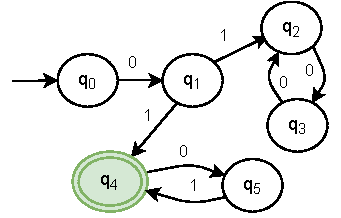
\includegraphics[]{diagrams-Original A.pdf}
	\caption{Non-deterministic finite automaton $A_1$.}
	\label{fig:NFA_A1_orig}
\end{figure}

NFA $A_1$ is a non-deterministic finite automaton (see state $q_1$) and uses multiple input symbols. Due to the fact we work with only recognized word lengths, we can substitute the automaton alphabet with a unary alphabet of a single input symbol $*$\footnote{Even though we do not actually need any particular input symbol, we use \emph{*} here as an example to depict the process. In general, all we need to know is that there is a transition between two states. The specific transition symbols are not significant for our optimization algorithm.}.

$$\Sigma = \{0, 1\} \longrightarrow \Sigma' = \{*\} $$

\begin{figure}[ht]
	\centering
	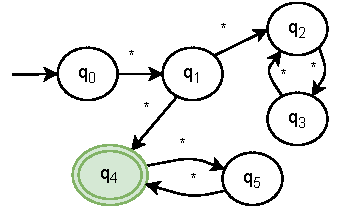
\includegraphics[]{diagrams-Original A Star.pdf}
	\caption{Non-deterministic finite automaton $A'_1$: $A_1$ with unified transition symbols.}
	\label{fig:NFA_A1_star}
\end{figure}

Then, we can generate \LSAa{$A_1$} for $A'_1$, which is its deterministic equivalent. For the final \LSAa{$A_1$}, generated from $A'_1$ by its determinization, see Figure~\ref{fig:HaL_A1}. \LSAa{$A_1$} accepts any words of lengths of words recognized by $A_1$. We will use these lengths in the process of constructing the product.

\begin{figure}[ht]
	\centering
	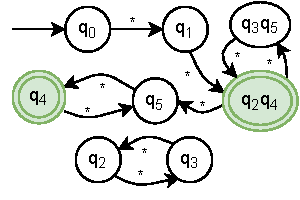
\includegraphics[]{diagrams-Final Handle and Loop Automaton A.pdf}
	\caption{Lasso automaton \LSAa{$A_1$} for the original NFA $A_1$ generated from $A'_1$ by its determination.}
	\label{fig:HaL_A1}
\end{figure}

You can notice \LSAa{$A_1$} looks different to what is depicted in Section~\ref{sec:length_abstraction}. It is caused by our optimization with generating only a single LSA per original automaton. \LSAa{$A_1$} is valid and the fact there are actually two separate automata with one even being inaccessible does not raise any issues for us. The reason for this behaviour will be further explained in Section~\ref{sec:singleHaL}.

The length abstraction formulae are generated for \LSAa{$A_1$}. For every state $q$, we get one or more existentially quantified formulae $\varphi$ in Presburger arithmetic describing language abstracting $\abstLA{q}$ in the form
\[
    \varphi: \exists k ( |w| = h + l \cdot k )
\]
where $|w|$ is a length of a recognized word, $h$ is the length of a handle to a certain final state $f$, and $l$ is the length of a loop to return to $f$ going through the loop. $k$ is the number of cycles through the loop states until a word ends in $f$. When multiple depicted formulae are created (because there are more final states or different accepting runs for a single final state in LSA resulting in multiple accepted lengths), we append these formulae with \emph{logical or}:
\[
    \alpha^{LA} : \exists k ( \varphi_1 \lor \ldots \lor \varphi_n )
\]
where $n$ is a number of generated $\varphi$.

%--------------------------------------------------------
%--------------------------------------------------------
\subsection{Single Lasso Automaton for Each Original Automaton}\label{sec:singleHaL}

When we are constructing a product $P$, we do not want to regenerate $\LSAa{A_1}$ and $\LSAa{A_2}$ for each new product state $p = [q_1, q_2]$. This is inefficient. Due to the nature of LSA, the successive product states $p'$ generate LSAs very similar to the LSAs for $p$. We just need to append new states to $Q_{LSA}$. As a result, we will work with only two lasso automata (possibly with multiple loops and/or multiple handles)---one for each automaton whose intersection is computed.

Therefore, our algorithm generates LSAs only once---state by state---checking every time, whether the new state $q$ is not already present in $Q_{LSA}$. If $q \notin Q_{LSA}$, we add $q$ to $Q_{LSA}$ and continue with the following states $q'$ until we either create an entirely new loop in LSA or generate $q' \in Q_{LSA}$. If $q' \in Q_{LSA}$, we can stop generating $q'$ as from now on, $\forall q' ( q' \in Q_{LSA})$.

%--------------------------------------------------------
%--------------------------------------------------------
\subsection{Product Construction with Length Abstraction Optimization}

To better demonstrate our solution, the second automaton we will be working with is a NFA $A_2$:
$$ A_2 = (\{s_0, s_1, s_2, s_3\}, \{0, 1\}, \delta_2, \{s_0\}, \{s_3\}) $$
where $\delta_2$ is depicted in Figure~\ref{fig:NFA_A2_orig}.

\begin{figure}[ht]
    \centering
	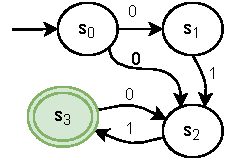
\includegraphics[]{diagrams-Original B.pdf}
	\caption{Non-deterministic finite automaton $A_2$.}
	\label{fig:NFA_A2_orig}
\end{figure}

In Figure~\ref{fig:HaL_A2}, there is \LSAa{$A_2$}, which we will be using together with \LSAa{$A_1$} shown in Figure~\ref{fig:HaL_A1} for computation of recognized word lengths.

\begin{figure}[ht]
    \centering
	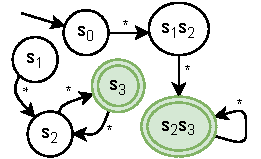
\includegraphics[]{diagrams-Final Handle and Loop Automaton B.pdf}
	\caption{Lasso automaton \LSAa{$A_2$} for the original NFA $A_2$.}
	\label{fig:HaL_A2}
\end{figure}

The core of the product construction algorithm remains unchanged, but there are a few differences. The Algorithm~\ref{productConstructionLengthAbstrAlg} shows how we alternate the original product construction algorithm to optimize the algorithm and resolve emptiness test for each \emph{branch} of the potential product automaton.

\begin{algorithm}
\caption{Product construction with length abstraction.}\label{productConstructionLengthAbstrAlg}
\SetKwInOut{Input}{Input}\SetKwInOut{Output}{Output}
\DontPrintSemicolon
\Input{ NFA $A_1 = (Q_1, \Sigma, \delta_1, I_1, F_1)$, NFA $A_2 = (Q_2, \Sigma, \delta_2, I_2, F_2)$}
\Output{ NFA $(A_1 \cap A_2) = (Q, \Sigma, \delta, I, F)$ with $L(A_1 \cap A_2) = L(A_1) \cap L(A_2)$}
\BlankLine
$Q, \delta, F \gets \emptyset$ \;
$I \gets I_1 \times I_2$ \;
$W \gets I$ \;\label{work_set}
$res \gets False$ \;\label{sat}
$solved \gets \emptyset$ \;\label{solved}
\While{$W \neq \emptyset$}{
    \textbf{picklast} $[q_1, q_2]$ \textbf{from} $W$\label{picklast} \;
    \textbf{add} $[q_1, q_2]$ \textbf{to} $solved$ \;
    $res \gets \abstLA{q_1} \land \abstLA{q_2} \textbf{ is } \emph{sat}$\label{satisfiable} \;
    \If{$res = True$}{\label{AlgSolveForSat}\label{satTrue}
        \textbf{add} $[q_1, q_2]$ \textbf{to} $Q$ \;
        \If{$q_1 \in F_1$ \textbf{and} $q_2 \in F_2$} {
        \textbf{add} $[q_1, q_2]$ \textbf{to} $F$ \;
        }\label{AlgAddToFinalState}
        \ForAll{$a \in \Sigma$}{
            \ForAll{$q'_1 \in \delta_1(q_1, a), q'_2 \in \delta_2(q_2, a)$}{
                \If{$[q'_1, q'_2] \notin solved$ \textbf{and} $[q'_1, q'_2] \notin W$}{
                    \textbf{add} $[q'_1, q'_2]$ \textbf{to} $W$ \;
                }
                \textbf{add} $[q'_1, q'_2] \textbf{ to } \delta([q_1, q_2], a)$ \;
            }
        }
    }
}
\end{algorithm}

We call $W$ from line \ref{work_set} a work set. It stores the potential product states prepared for processing, which we pick from $W$ one by one\footnote{In spite of the fact more approaches are valid, we strongly recommend picking the last added product state from $W$ (see line \ref{picklast})---using depth-first search---as this allows us to quickly advance through the automaton and get to any final state faster---in case we just want to know whether automata have a non-empty intersection, this change will get us the answer most of the time in less steps. It works even better when implemented with a satisfiable state skipping optimization, explained in Section~\ref{sec:skipping states}.}.

The optimization process starts when we pick a product state $p$ from $W$. Instead of immediately generating new successive product states $p'$, we test $p$ for satisfiability of length constraints of recognized words from $p$: $\sat{\compatLA{p}}$ where
\[
    \compatLA{p} : \abstLA{q_1} \wedge \abstLA{q_2} \text{ and}
\]
$\sat{\psi}$ is \emph{True} iff $\psi$ is satisfiable ($\Phi \textbf{ is } \emph{sat}$), $False$ otherwise. On line \ref{satisfiable}, we check whether $\sat{\compatLA{p}}$ holds. If $\sat{\compatLA{p}}$, i.e., there will be an accepting run using $p$ (see line \ref{satTrue}), we add $p$ to $Q$, possibly to $F$ and generate $p'$.

We start with initial states and make our way through both automata as we progress with successive product states. For each $p$, we set initial states in both LSAs to the respective corresponding states in $p$. For $p = [q_0, s_0]$, we get the following length abstraction formulae. From \LSAa{$A_1$} for $q_0$ (as a new initial state of $\LSAa{A_1}$), we get an existential formula representing length abstraction $\abstLA{q_1}$\footnote{This formula consists of two independent disjuncts $\varphi_1$ and $\varphi_2$ describing there are more possible lengths for accepted words from the same initial state (leading to two independent final states in the automaton).}. From \LSAa{$A_2$} for $s_0$ (as a new initial state of $\LSAa{A_2}$), we get a formula for length abstraction $\abstLA{s_0}$\footnote{We are using variable $m$ here instead of $k$ to emphasize variables from different formulae are not dependent on each other---they belong to different LSAs.}.
\begin{align*}
    &\abstLA{q_0}: \exists k ( |w| = 2 \lor |w| = 4 + 2 \cdot k ) \\
    &\abstLA{s_0}: \exists m ( |w| = 2 + 1 \cdot m )
\end{align*}

When we compare $\abstLA{q_0}$ and $\abstLA{s_0}$, we get:
\[
    \abstLA{q_0} \land \abstLA{s_0} : \exists k ( |w| = 2 \lor |w| = 4 + 2 \cdot k ) \land \exists m ( |w| = 2 + 1 \cdot m )
\]
or in a simplified notation:
$$ \abstLA{q_0} \land \abstLA{s_0} : \exists k \exists m ( 2 \lor 4 + 2 \cdot k = 2 + 1 \cdot m ) $$

We try to find values of $k$ and $m$ such that $|w|$ equal (some expressions on the left and on the right side of the equation are equal). We pass this formula to an SMT solver to solve its satisfiability. SMT solver returns \emph{sat} when satisfiable ($res$ is set to \emph{True}) and \emph{unsat} when unsatisfiable ($res$ is set to \emph{False}). If \emph{unsat} is returned, we can stop generating this \emph{branch} of a NFA as we know for sure there cannot be a word which is accepted by both $A_1$ and $A_2$, when there is even no word fulfilling the length requirements. In this case, we have successfully reduced the generated state space by omitting the product state $p$ and any further product states $p'$, which would be later normally generated from $p$ and its successors (assuming the transition symbols correspond).

The $\alpha^{LA}$ compatibility check $\sat{\compatLA{p}} = \abstLA{q_1} \land \abstLA{q_2} \textbf{ is } \emph{sat}$ can be implemented in SMT solver as in Algorithm~\ref{checkLengthAbstractionSatisfiabilitySMTAlgorithm}:

\begin{algorithm}
\newcommand{\LAFormula}[1]{\varphi_{#1}}

\caption{Check length abstraction compatibility with SMT solver.}\label{checkLengthAbstractionSatisfiabilitySMTAlgorithm}
\SetKwInput{Input}{Input}
\SetKwInput{Output}{Output}
\SetKw{Return}{return}
\SetKw{Break}{break}
\SetKwFunction{FIsLengthAbstractionSatisfiable}{isLengthAbstractionSatisfiable}
\SetKwFunction{FSMTInit}{smtInit}
\SetKwFunction{FSMTAdd}{smtAdd}
\SetKwFunction{FSMTPush}{smtPush}
\SetKwFunction{FSMTPop}{smtPop}
\SetKwFunction{FSMTCheck}{smtCheck}
\SetKwProg{Fn}{Function}{:}{}

\DontPrintSemicolon
\BlankLine

$\FSMTInit{}$ \;
$\FSMTAdd{$k \geq 0, m \geq 0$}$ \;

\For{$\LAFormula{q_1} \in \abstLA{q_1}$}{
    \For{$\LAFormula{q_2} \in \abstLA{q_2}$}{
        $\FSMTPush{}$ \;
        $\FSMTAdd{$\LAFormula{q_1}.handle + \LAFormula{q_1}.lasso * k = \LAFormula{q_2}.handle + \LAFormula{q_2}.lasso * m$}$ \;
        $res \gets \FSMTCheck{}$ \;
        \If{$res = True$}{
            \Break \;
        }
        $\FSMTPop{}$ \;
    }
}
\end{algorithm}



In Figure~\ref{fig:product_WIP}, we can see the product of $A_1$ and $A_2$ being constructed using length abstraction optimization. Red states represent tested states that are resolved as unsatisfiable for computed length formulae and therefore the algorithm omits any successive product states---dashed states (such as $q_4s_2$ or $q_3s_2$) which are generated in the basic naive product construction algorithm. The green state represents final states in both automata. Here, we have found a possible solution accepted by both original automata. If we desire to resolve only the product emptiness test, we can stop the execution of the algorithm here as we have found one final state---automata have non-empty intersection. The blue state is a normal product state whose significance will be explained in section~\ref{sec:skipping states}.

\begin{figure}[ht]
	\centering
	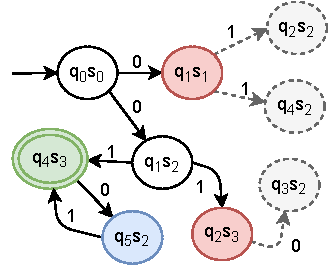
\includegraphics[]{diagrams-skip WIP Product .pdf}
	\caption{Constructed product automaton with depiction of length abstraction optimization.}
	\label{fig:product_WIP}
\end{figure}

As you can notice in Figure~\ref{fig:product_final}, the product generated by our algorithm has only 4 product states in comparison to 9 product states generated by the classic algorithm.

\begin{figure}[ht]
	\centering
	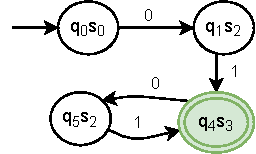
\includegraphics[]{diagrams-Final Product.pdf}
	\caption{Final product generated by product construction algorithm minimized by length abstraction optimization by omitting unnecessary states on the fly.}
	\label{fig:product_final}
\end{figure}


When we get $\neg \sat{\compatLA{p}}$, we do not need to construct any following states $p'$ and check whether $\sat{\compatLA{p'}}$. Therefore, we are able to determine whether such \textit{branches} of automata have an empty intersection and we do not need to consider them in the product construction. The emptiness test is successfully accomplished, and we determined that for this \emph{branch} there cannot exist any word accepted by both automata and consequently by their intersection. When we get unsatisfiable result for every branch of the automaton (i.e., no \emph{branch} can lead to any final state) even if by inspecting transition symbols it looks like there could be a non-empty intersection, we can say that such input automata have an empty intersection and product construction will be very quick in that case---this is where our optimization dominates.

A note of caution. It is important to understand that we are working only with possible word lengths and when we test the emptiness of intersection of automata, we can resolve only such intersections that words lengths are not accepted by both automata. When the test shows there could be some words of certain length accepted by both automata and for that reason by their intersection too---$\sat{\compatLA{p}}$---we cannot be sure there truly are any words accepted by both automata with their intersection non-empty, because there may be words of the suggested length, but it may be a different word for each automaton (which differ from one another in the containing symbols or their position in the word). For resolving such cases, we have to proceed with the classic algorithm steps to produce product states according to their original transition symbols, not only by comparing the possible words lengths. With certainty, we can omit only the cases where $\neg \sat{\compatLA{p}}$.

%--------------------------------------------------------
%--------------------------------------------------------

\subsection{Optimization with Skipping Satisfiable States} \label{sec:skipping states}

When we take new $p$ from $W$ and check whether $\sat{\compatLA{p}}$, it is time to add all the possible successive product states $p'$ to $W$. When $p$ generates only a single $p'$, we can say with certainty that $\sat{\compatLA{p'}}$ as there is only a single branch in the automaton leading from $p$ to a~final state (through $p'$). $p'$ is \emph{skippable}, iff there exists $p$ for which $\sat{\compatLA{p}}$ and whose only successor is $p'$. We add $p'$ to $W$ with the information of being skippable. If $p'$ is already in~$W$, we append the information to $p'$ in $W$.

We skip checking for $\sat{\compatLA{p'}}$ when we pick $p'$ from $W$. We can immediately check for final states and generate the successive product states. This optimization saves us generating the length abstraction formulae for $p'$ and testing the formulae in the SMT solver for their satisfiability and even possibly reducing the number of states generated for both initial automata.

If automata have long lines (with non-splitting branches), this will prove extremely useful, because only a few proper iterations with formulae computing and executing SMT solver will be executed. The application of skipping satisfiable states is depicted in Algorithm~\ref{productConstructionLengthAbstrAlgSkip}. The line~\ref{satisfiable} from Algorithm~\ref{productConstructionLengthAbstrAlg} is substituted with the contents of Algorithm~\ref{productConstructionLengthAbstrAlgSkip}.

%{ \LinesNotNumbered
\begin{algorithm}
\SetKwFunction{FSkippable}{skippable}
\SetKwFunction{FSatisfiable}{satisfiable}
    \caption{Substitution of line~\ref{satisfiable} in Algorithm~\ref{productConstructionLengthAbstrAlg} with skipping satisfiable states.} \label{productConstructionLengthAbstrAlgSkip}
    \DontPrintSemicolon
    \eIf{$ \FSkippable{$[q_1, q_2]$}$}{
        $res \gets True$ \;
    }{
        $res \gets \abstLA{q_1} \land \abstLA{q_2} \textbf{ is } \emph{sat}$ \;
    }
\end{algorithm}
%}

The only change is a test for every checked $p$, which decides whether $p$ can be skipped. You can see that we proceed with SMT solver satisfiability check only for $p$ which are generated from the product states with multiple transitions generating $p$ and at least one more product state (in general at least two new potential product states). If only one $p$ was generated earlier from a product state with satiafiable formulae of non-zero length\footnote{If the satisfiable length is zero, we are in a final product state and $p$ generated from final state might not lead to any final state, but the length abstractions for final state are compatible, of course.}, we skip the check for $\sat{\compatLA{p}}$ and continue to generating its successive states immediately.

You can notice there is one skippable state in the former example, which had to be evaluated and tested for satisfiability earlier. The blue state in Figure~\ref{fig:product_WIP} is such a skippable state. In our case for state $q_5s_2$, when only one new state is generated from state $q_4s_3$ while this state is resolved as satisfiable (with non-zero length---otherwise, if $q_5s_2$ did not lead back to $q_4s_3$, $q_5s_2$ would be skippable even though it would not lead to any final state), newly generated product state has to be satisfiable as well, because the check for $q_4s_3$ already considered the state $q_5s_2$ as its only way to any final state with non-zero length.

When we have a series of such states, we can highly optimize generating the whole branch with only one initial check for satisfiability. In real world examples, there are often automata with long branches splitting into multiple branches only occasionally. We will check for satisfiability for all the initial states of each new branch and then either omit the entire branch (if \emph{unsat} is returned) or skip checking satisfiability in the entire branch (if \emph{sat} is returned).

\subsection{Resolving Length Abstraction Satisfiability without SMT Solver}

The structure of length abstraction formulae allows us to compute their satisfiability without the need to use SMT solvers\footnote{Note that, as with SMT solver, we do not need to find specific values for which the formulae are satisfiable. We are only interested in deciding whether such values exist.}. $\compatLA{p}$ forms a set of linear congruence equations, which can be resolved just by utilizing basic maths operations and linear congruence qualities.

The Algorithm~\ref{checkLengthAbstractionSatisfiabilitySMTFreeAlgorithm} shows how to determine $\sat{\compatLA{p}}$ from line~\ref{satisfiable} without an SMT solver.

% TODO: Comment on SMT solver removal for length abstraction.

\begin{algorithm}
\newcommand{\LAFormula}[1]{\varphi_{#1}}

\caption{Check satisfiability using length abstraction algorithm without SMT solver.}\label{checkLengthAbstractionSatisfiabilitySMTFreeAlgorithm}
\SetKw{Return}{return}
\SetKwFunction{FIsLengthAbstractionSatisfiable}{isLengthAbstractionSatisfiable}
\SetKwFunction{FSolveForOneHandleLonger}{solveForOneHandleLonger}
\SetKwFunction{FGetGCD}{getGCD}
\SetKwProg{Fn}{Function}{:}{}

\DontPrintSemicolon
% The function code itself.
\For{$\LAFormula{q_1} \in \abstLA{q_1}$}{
    \For{$\LAFormula{q_2} \in \abstLA{q_2}$}{
        \uIf{$\LAFormula{q_1}.handle = \LAFormula{q_2}.handle$}{
            $res \gets True$ \;
        } \uElseIf{$\LAFormula{q_1}.handle > \LAFormula{q_2}.handle$}{
            $res \gets \FSolveForOneHandleLonger{$\LAFormula{q_1}$, $\LAFormula{q_2}$}$ \;
        } \uElse{
            $res \gets \FSolveForOneHandleLonger{$\LAFormula{q_2}$, $\LAFormula{q_1}$}$ \;
        }
    }
}

$res \gets False$ \;
\end{algorithm}

We execute the following steps for each equation
\[
    \varphi_{q_1}.handle + \varphi_{q_1}.lasso \cdot k = \varphi_{q_2}.handle + \varphi_{q_2}.lasso \cdot m \text{.}
\]

If the handle lengths of $\varphi_{q_1}$ and $\varphi_{q_2}$ are equal, there are words of the same length accepted by both $\abstLA{q_1}$ and $\abstLA{q_2}$ (they are mutually compatible) without stepping into the loops of \LSAa{$A_1$} and \LSAa{$A_2$}. Otherwise, handle lengths differ, and we must consider lengths of loops in our determination of compatibility of $\abstLA{q_1}$ and $\abstLA{q_2}$.

We now have to determine $\sat{\varphi_{q_1} \land \varphi_{q_2}}$ for abstractions with one handle longer. This is solved by the function \texttt{solveForOneHandleLonger} in Algorithm~\ref{checkLengthAbstractionSatisfiabilitySMTFreeAlgorithmFunctionImplementation}.

\begin{algorithm}[ht]
\newcommand{\LAFormulaLonger}{\varphi_{l}}
\newcommand{\LAFormulaShorter}{\varphi_{s}}
\newcommand{\HandleDifference}{\LAFormulaLonger.handle}
\newcommand{\CurrentIteration}{it}

\caption{Solve satisfiability of length abstraction formulae for one handle longer.}\label{checkLengthAbstractionSatisfiabilitySMTFreeAlgorithmFunctionImplementation}
\SetKw{Return}{return}
\SetKwFunction{FIsLengthAbstractionSatisfiable}{isLengthAbstractionSatisfiable}
\SetKwFunction{FSolveForOneHandleLonger}{solveForOneHandleLonger}
\SetKwFunction{FGetGCD}{getGCD}
\SetKwProg{Fn}{Function}{:}{}

\DontPrintSemicolon
\Fn{\FSolveForOneHandleLonger{$\LAFormulaLonger$, $\LAFormulaShorter$}}{
    \KwData{
    Input length abstraction formulae of potential product state.\\
    $\LAFormulaLonger$: Length abstraction formula with the longer handle, \\
    $\LAFormulaShorter$: Length abstraction formula with the shorter handle.
    }
    \KwResult{bool: \emph{True} if satisfiable, \emph{False} otherwise.}

    % The function code itself.
    $\HandleDifference \gets \LAFormulaLonger.handle - \LAFormulaShorter.handle$ \label{simplifyEquation} \;
    $\LAFormulaShorter.handle \gets 0$ \;

    \uIf{$\LAFormulaLonger.lasso = 0 \textbf{ and } \LAFormulaShorter.lasso = 0$}{\label{both_no_loops}
        \Return $False$ \;
    } \uElseIf{$\LAFormulaShorter.lasso = 0$}{\label{shorter_no_loop}
        \Return $False$ \;
    } \uElseIf{$\LAFormulaLonger.lasso = 0$}{\label{longer_no_loop}
        $\CurrentIteration \gets 0$ \tcp*[h]{Current length resembling the iteration of the shorter lasso loop.} \;
        \While{$\CurrentIteration \leq \HandleDifference$}{
            \eIf{$\CurrentIteration = \HandleDifference$}{
                \Return $True$ \;
            }{
                $\CurrentIteration \gets \CurrentIteration + \LAFormulaShorter.lasso$ \;
            }
        }
        \Return $False$ \;
    } \uElse{\label{both_loops}
        $gcd \gets \FGetGCD{$\LAFormulaLonger.lasso$, $\LAFormulaShorter.lasso$}$ \;
        \eIf{$gcd = 1$}{
            \Return $True$ \;
        }{
            $y \gets - \HandleDifference$ \;
            \While{$y < gcd$}{
                $y \gets y + \LAFormulaShorter.lasso$ \;
            }
            \eIf{$(y \mod gcd) = 0$}{
                \Return $True$ \;
            } {
                \Return $False$ \;
            }
        }
    }
}
\end{algorithm}

First, to simplify the equation (line~\ref{simplifyEquation}), we move handle lengths from the side of the equation with the shorter handle $\varphi_s$ to the side with the longer handle $\varphi_l$ to solve:
\begin{equation}\label{simplified_equation}
    \varphi_{l}.handle + \varphi_{l}.lasso \cdot k = \varphi_{s}.lasso \cdot m
\end{equation}
which represents the number of loops a word must make in $\varphi_{s}$ to be accepted by $\varphi_l$ (as if with shorter $\varphi_l.handle$).

If both $\varphi_l$ and $\varphi_s$ have no loops (line~\ref{both_no_loops}), $\varphi_{q_1} \land \varphi_{q_2}$ is unsatisfiable because the handles differ. Else, if only $\varphi_s$ has no loop (line~\ref{shorter_no_loop}), every word accepted by $\varphi_s$ is shorter than words accepted by $\varphi_l$ and the formulae cannot be satisfiable.

Else, if only $\varphi_l$ has no loop (line~\ref{longer_no_loop}), we can try to manually iterate over loops in $\varphi_s$ to see whether the word length difference between handles can be equalized by looping in $\varphi_s.lasso$.

Otherwise, both $\varphi_l$ and $\varphi_s$ have loops (line~\ref{both_loops}). We can apply linear congruence qualities to the equation~\ref{simplified_equation} to determine whether the formulae are satisfiable. The equation~\ref{simplified_equation} says that if formulae are satisfiable, the left side of the equation is divisible by some multiple of $\varphi_s.lasso$. We can rewrite that in a linear congruence as follows:
\begin{align}
    \varphi_{l}.handle + \varphi_{l}.lasso \cdot k &\equiv 0 \pmod{\varphi_s.lasso} \\
    \varphi_{l}.lasso \cdot k &\equiv - \varphi_{l}.handle  \pmod{\varphi_s.lasso} \label{linear_congruence_equation}
\end{align}
which is the same as solving a linear Diophantine equation
\begin{equation}
    \varphi_{l}.lasso \cdot k - \varphi_s.lasso \cdot m = - \varphi_{l}.handle \text{.} \label{linear_diophantine_equation}
\end{equation}

Qualities of multiplicative inverse~\cite{DivisibilityAndGreatestCommonDiviser, LinearCongruences}, based on Bézout's identity~\cite{DivisibilityAndGreatestCommonDiviser}, say that iff $\varphi_l.lasso$ and $\varphi_s.lasso$ are relatively prime (coprime)---the greatest common divisor (GCD) of $\varphi_l.lasso$ and $\varphi_s.lasso$ is equal to $1$---there exists a multiplicative inverse for $\varphi_l.lasso$ in modulo $\varphi_s.lasso$ which ensures that linear congruence~\ref{linear_congruence_equation} is always solvable for some $\varphi_l.lasso$ in modulo $\varphi_s.lasso$\footnote{We can get the precise solution by multiplying both sides of the equation with the multiplicative inverse.}. Therefore, the formulae are satisfiable.

Otherwise, $\varphi_l.lasso$ and $\varphi_s.lasso$ are not coprime (GCD is different from $1$) and by qualities of linear Diophantine equations~\cite{LinearCongruences}, iff GCD precisely divides $y$ without a remainder where $y$ is the right side of the linear congruence~\ref{linear_congruence_equation} or its any congruent equivalent, there exist solutions to the linear congruence\footnote{We can apply extended Euclidean algorithm to find the precise values for the Diophantine equation~\ref{linear_diophantine_equation}.}. Otherwise, there are no solutions.

%--------------------------------------------------------
%--------------------------------------------------------
%--------------------------------------------------------
%--------------------------------------------------------
\section{Parikh Image Abstraction of State Languages}

$\abstLA{q}$ is a simple and fast optimization, but can be too general to detect non-terminating states in some cases. In this section, we present a product construction optimization using Parikh image state language abstraction, which aims to make the abstraction more accurate to prune larger quantities of unnecessary generated product state space.

Parikh images provide more information about the finite automata than simple length abstraction. While length abstraction considers only accepted word lengths without knowing which transition symbols are actually in the transitions, Parikh image abstracts accepted words to numbers of occurrences of specific transition symbols in words regardless of their position in words. Thus, Parikh image abstraction allows us to more precisely determine the emptiness of finite automata intersection. However, Parikh image computation itself consumes a considerate amount of computational time for larger finite automata. The question is, whether the added computation time compensates for more precise product generation with higher product states pruning capabilities.

We introduce an algorithm for Parikh image computation applied on each potential product state $p = [q_1, q_2]$ to decide the compatibility of its $\abstPI{q_1}$, $\abstPI{q_2}$ (mutual satisfiability of formulae describing the abstractions). If the abstractions are proved to be compatible, $p$ is added to the generated product. Otherwise, $p$ is omitted and no additional $p'$ such that $p' = \delta(p, a)$ accessible only from $p$ are added to the queue to test their abstractions' compatibility. Generalization to n-tuples is then a matter of adding additional abstraction equal to the number of input automata.

\subsection{Parikh Image} \label{sec:parikhImage}

We derive our Parikh image construction from the Parikh's theorem~\cite{Kozen1977} described in~\cite{ParikhsTheoremSimpleAndDirectConstruction}, creating a semi-linear Parikh image formulae for the given regular language as a set of Parikh images for each word in the language. However, our usage of Parikh image of some regular language (and therefore of the corresponding finite automaton recognizing such regular language) is restricted to determining the compatibility of Parikh image state language abstractions. Therefore, we only test for satisfiability of Parikh image formulae describing $\abstPI{q_i}$. We use SMT solver to resolve the satisfiability of Parikh image formulae of the current potential product state.

Our Parikh image formulae consist of the following constraints, in conjunctive normal form. For each potential product state, there exists exactly one our formula of Parikh image describing its regular language. We ask the SMT solver whether the Parikh image constraints for corresponding states in the original automata (one state per automaton) are compatible with each other. This ensures that we construct only those product states which satisfy the Parikh image constraints, otherwise we deem such potential product states redundant and such states can be pruned.

Given an NFA $A = (Q, \Sigma, \Delta, I, F)$ where $I$ is a singleton $I = \{ q_{0} \}$, Parikh image formula $\varphi$ (as described in~\cite{PI_computation/10.1007/978-3-030-45093-9_59} for solving string constraints) consists of the following conjuncts. $\varphi$ describes runs of $A$ (precisely, their over-approximation). The defined variables represent qualities of each run, their precise values the precise qualities of the specific run. Satisfiable assignment defines a set of runs with qualities given by the assigned variable values.

\begin{enumerate}
    \item \label{clauses:u_original} Foremost, we define a variable $u_{q}$ for each state $q \in Q$. $u_{q}$ defines how many times we enter $q$ and exit $q$ again by specifying the difference between the number of entries and exits. We construct equations with $u_{q}$ for a run as follows:
    \begin{itemize}
        \item $u_{q} = 1$ for $q \in I$,
        \item $u_{q} \in \{ 0, -1 \}$ for $q \in F$ and
        \item $u_{q} = 0$ for $q \in Q \setminus ( I \cup F )$.
    \end{itemize}

    \item \label{clauses:y_original} Second, we define a variable $y_{t}$ for each transition $t \in \Delta$ such that $y_{t} \geq 0$ describing how many times is $t$ used in the run.

    \item \label{clauses:uy_original} We can now present an equation introducing a connection between $u_{q}$ and $y_{t}$ to evaluate the difference between the number of entries and exits for each $q \in Q$ as follows:
    $$ u_q + \sum_{t \in \Delta_q^+} y_t - \sum_{t \in \Delta_q^-} y_t = 0.$$
    where $\Delta_q^+$ is a set of ingoing transitions $ \Delta_q^+ = \{ (q',a,q) \in \Delta \}$ and $\Delta_q^-$ is a set of outgoing transitions $ \Delta_q^- = \{ (q,a,q') \in \Delta \} $ from the given state $q$.

    \item \label{clauses:hash_original} Furthermore, we declare the only free variable $\#_a$ for each transition symbol $ a \in \Sigma$. $\#_a$ describes the number of occurrences of $a$ in accepted words regardless of their position in the words (the number of $a$ in the run). The constraint $\#_a = \sum_{t = (q, a, q') \in \Delta} y_t$ ensures $\#_a$ is consistent with the number of used $t$ with $a$.

    \item \label{clauses:z_original} Last, but not least, we make sure the regular language expressed by Parikh image preserves the connectedness of $A$---the used automata states are accessible from $I$ and they are connected by transitions. Variable $z_q$ for each $q \in Q$ is introduced. $z_q$ represents the length of the path from $I$ to $q$ in a spanning tree of the subgraph with $y_t \geq 0$.

    If $q \in I$, we add a constraint $z_q = 1 \land y_t \geq 0$. Otherwise,
    {
    \begin{align*}
        (z_q = 0 \land \bigwedge_{t \in \Delta_q^+} y_t = 0) \lor \bigvee_{t \in \Delta_q^+} (y_t \geq 0 \land z_{q'} \geq 0 \land z_q = z_{q'} + 1) \text{.}
    \end{align*}
    }
    If the distance $z_q$ is $0$, $q$ is not in the run.
\end{enumerate}

We gain an existentially quantified formula $\varphi$ in Presburger arithmetic describing language abstracting $\alpha^{PI}$ for $A$ with free variables $\#_a$:
$$ \alpha^{PI} : \exists u_{q_1},\ldots,u_{q_n},z_{q_1},\ldots,z_{q_n},y_{t_1},\ldots,y_{t_m} ( \varphi ) $$
where $n = \lvert Q \rvert$ is the number of states and $m = \lvert \Delta \rvert$ is the number of transitions in the finite automaton.

For SMT solving, it is paramount that we have formulae without universal quantifiers, otherwise the SMT solver computation could \emph{explode} computation time-wise. SMT solver work best with quantifier-free or existential formulae. Thanks to how Parikh image is constructed, our approach takes advantage of these SMT qualities and our Parikh image formulae can be inserted in SMT solver as quantifier-free.

\subsection{Reduced Parikh Image}\label{sec:reducedParikhImage}

The presented Parikh image works as intended. Nevertheless, the described Parikh image computation requires extensive resources and computation time. However, we use Parikh image only for determining the emptiness of the product. Given that most of the computation time is taken by the evaluation of these conjuncts, we try to minimize the number of Parikh image formula conjuncts SMT solver needs to evaluate for each $\varphi$.

Consequently, we infer our reduced Parikh image from the above shown Parikh image to further optimize Parikh image computation. We strip Parikh image of for our purposes unnecessary constraints and unify initial states as well as accept states.

%TODO Unification of inital and accept states

Our reduced Parikh image consists of the following conjuncts:
\begin{enumerate}
    \item \label{clauses:u_reduced} We use the conjuncts~\ref{clauses:u_original}, except now we restrict $u_q$ for each final state to have only the value $-1$, i.e.:
    $$ u_{q} = -1 \text{ for each state } q \in F \text{.}$$

    We can perform this reduction, because we know for sure that by unifying final states of the automaton into one abstract final state, there will be exactly only one final state where all words accepted by the automaton end, but none passes through this state earlier.
    %TODO Why to change this? Cannot it be only the single one? Is it because of the unified initial and final state.

    \item \label{clauses:y_reduced} \label{clauses:uy_reduced} \label{clauses:hash_reduced} The conjuncts~\ref{clauses:y_original} and~\ref{clauses:uy_original} remain unchanged, the same holds for conjuncts~\ref{clauses:hash_original}.
    \item \label{clauses:z_reduced} However, we completely omit the conjuncts for $z_{q}$ which ensure the connectedness of the Parikh image representation of finite automaton. The reason is that, as we have found out, the difference in pruning capabilities of Parikh image with or without the conjuncts~\ref{clauses:z_original} on our benchmark automata is insignificant in comparison to the computation time spared by removing these conjuncts %TODO: Add experiments there: (see Section~\ref{sec:experiments_and_results}).

    The reason conjuncts~\ref{clauses:z_original} are so demanding computation time-wise is that all these conjuncts have to be always recomputed for each single state Parikh image is computed for. Furthermore, the conjuncts themselves are complex for even simple automata. For that reason, SMT solvers need extensive resources to compute Parikh images with these conjuncts in consideration.

    Even then, if we require ensuring that the reduced Parikh image represents the connectedness of the finite automaton, we can include these conjuncts, but, thanks to our unification of initial and accept states, we change them as follows to reflect our initial and accept state unification changes:

    The constraint for when $q$ is an initial state ($z_q = 1 \land y_t \geq 0$) remains unchanged. However, for every other state, we remove the possibility of $y_t = 0$ and $z_{q'} = 0$ in the second half of the conjuncts. The conjuncts look like this:
    {
    \begin{align*}
		(z_q = 0 \land \bigwedge_{t \in \Delta_q^+} y_t = 0) \lor \bigvee_{t \in \Delta_q^+} (y_t > 0 \land z_{q'} > 0 \land z_q = z_{q'} + 1) \text{.}
    \end{align*}
    }

\end{enumerate}

Our goal is to reduce the number of conjuncts the SMT solver needs to compute for each potential product-state. We focus on several optimizations such as incremental SMT solving,

Due to how we have reduced our Parikh image used for automata state language abstraction, we work only with finite automata with a single initial state and a single accept state. However, we can easily convert any finite automaton into the required format with adding two new states to each input automaton. One for a new initial state from which one can transition to all previous initial states and one for a new accept state to which lead all previous accept states. The previous initial and accept states are changed to common automata states.

% TODO Algorithm or pseudocode? What about? Formal math representation?

\subsubsection{Compatibility of Multiple Parikh Image State Language Abstractions}

So far, we have shown how to compute Parikh image for a single finite automaton to represent said automaton with a single formula. We want to use this formula in such a way that would allow us to decide satisfiability of those formulae for multiple automata simultaneously when the formulae are combined into a single formula which we can decide its satisfiability for. The following paragraphs show how we use these features of Parikh images to determine satisfiability of multiple Parikh image formulae.

We can compute $\varphi_1$ for $A_1$ and $\varphi_2$ for $A_2$. Each $\varphi_i$ represents exactly one $A_i$. Therefore, each $\varphi_i$ by itself is satisfiable for $A_i$ where $\varphi_i$ describes words accepted by $A_i$\footnote{Our Parikh image is an over-approximation of the accepted language of $A_i$. Therefore, there could exist such evaluation of variables in $\varphi_i$ which describes words not accepted by $A_i$. It is a trade-off of precise representation of $A_i$ for faster computation of $\varphi_i$.}.

If each $\varphi_i$ is satisfiable, we want to know whether a combination of state language abstractions is compatible at the same time: $\sat{\compatPI{p}}$ such that $p = [q_1, q_2]$ is a product state and
\[
    \compatPI{p} : \abstPI{q_1} \wedge \abstPI{q_2} \text{.}
\]

However, to maintain the languages of specific automata distinguishable, we label each variable $u_q, y_t$ (optionally, $z_q$, too) for each $\varphi_i$ according to $i$: $u_{iq}, y_{it}$ ($z_{iq}$). The only exception are free variables $\#_a$ which in contrary are bound to transition symbols $a \in \Sigma$ common to both $A_i$.

$\sat{\compatPI{p}}$ means there are words accepted by all $\varphi_i$ simultaneously and therefore by both $A_i$. Consequently, the automata product would be non-empty.

\subsection{Product Construction with Parikh Image Abstraction Optimization}

We introduce the basic algorithm using Parikh image computation to construct the product of the intersection of finite automata. The algorithm resembles the length optimization algorithm from Algorithm~\ref{productConstructionLengthAbstrAlg}. However, we compute Parikh image formulae and determine their satisfiability instead of generating lasso automata and determining satisfiability of length abstraction formulae now to optimize product construction.

We use Parikh image formulae to determine whether $p$ is to be added to the generated product $P$ (in case $\sat{\compatPI{p}}$) or omitted (in case $\varphi_1$ and $\varphi_2$ are unsatisfiable simultaneously in $\compatPI{p}$.

We can see our proposed algorithm using Parikh image computation to optimize product construction in the Algorithm~\ref{productConstructionParikhImageAlgorithm}. Similarly to the length abstraction algorithm, we start with the initial states (our abstract initial state, as described in Section~\ref{sec:reducedParikhImage}) of $A_1$ and $A_2$, compute $\varphi_1$ and $\varphi_2$ combined into a single formula $\compatPI{p}$. If $\neg \sat{\compatPI{p}}$, $P$ is empty and we can stop the product generation at once. Otherwise, $\sat{\compatPI{p}}$ is satisfiable and the corresponding product state is added to $P$. We proceed to generate the consecutive potential product states. We set the initial states for Parikh image formulae computation to the current state for each automaton $A_i$ for each potential product state and recompute the combined Parikh image formula. We iterate over potential product states from $W$ (see line~\ref{PIAlgorithm:IterateOverProductStates}).

The expression in line~\ref{areParikhImageFormulaeSatisfiable} computes state language abstractions by computing Parikh image formulae, determines their compatibility (satisfiability of Parikh image formulae) and returns the result as a boolean value. We are only interested in the satisfiability test result because we do not need any additional information from the computed formulae. Therefore, a simple boolean value is sufficient. The result of the satisfiability test is used further in the algorithm to determine whether the product state is added to the generated product and consecutive potential product states are appended to $W$. The Parikh image is computed as it is explained in Section~\ref{sec:reducedParikhImage}.

\begin{algorithm}
\caption{Product construction algorithm with Parikh image abstraction.}\label{productConstructionParikhImageAlgorithm}
\SetKwInOut{Input}{Input}
\SetKwInOut{Output}{Output}
\SetKwFunction{FStateAbstractionPI}{$ \alpha^{PI} $}
\DontPrintSemicolon
\Input{ NFA $A_1 = (Q_1, \Sigma, \delta_1, I_1, F_1)$, NFA $A_2 = (Q_2, \Sigma, \delta_2, I_2, F_2)$}
\Output{ NFA $P = (A_1 \cap A_2) = (Q, \Sigma, \delta, I, F)$ with $L(A_1 \cap A_2) = L(A_1) \cap L(A_2)$}
\BlankLine
$Q, \delta, F \gets \emptyset$ \;
$I \gets I_1 \times I_2$ \;
$W \gets I$ \;
$res \gets False$ \;
$solved \gets \emptyset$ \;\label{PIAlgorithm:solved}
\While{$W \neq \emptyset$}{\label{PIAlgorithm:IterateOverProductStates}
    \textbf{picklast} $[q_1, q_2]$ \textbf{from} $W$ \;
    \textbf{add} $[q_1, q_2]$ \textbf{to} $solved$ \;

    $res \gets \FStateAbstractionPI{$q_{1}$} \land \FStateAbstractionPI{$q_{2}$} \textbf{ is } \emph{sat} $ \label{areParikhImageFormulaeSatisfiable} \;

    \If{$res = True$}{
        \textbf{add} $[q_1, q_2]$ \textbf{to} $Q$ \;
        \If{$q_1 \in F_1$ \textbf{and} $q_2 \in F_2$} {
        \textbf{add} $[q_1, q_2]$ \textbf{to} $F$ \;
        }
        \ForAll{$a \in \Sigma$}{
            \ForAll{$q'_1 \in \delta_1(q_1, a), q'_2 \in \delta_2(q_2, a)$}{
                \If{$[q'_1, q'_2] \notin solved$ \textbf{and} $[q'_1, q'_2] \notin W$}{
                    \textbf{add} $[q'_1, q'_2]$ \textbf{to} $W$ \;
                }
                \textbf{add} $[q'_1, q'_2] \textbf{ to } \delta([q_1, q_2], a)$ \;
            }
        }
    }
}
\end{algorithm}

\subsubsection{Skippable States Optimization}

Same as for the length abstraction, we can make use of skipping satisfiable product states optimization. When $\sat{\compatPI{p}}$ for some potential product state $p = [q_1, q_2]$ and $p$ generates only one consecutive potential product state $p' = [q^{'}_1, q^{'}_2]$ such that $p \rightarrow{a} p'$ where $ a \in \Sigma $, we can skip computing Parikh images for $p'$ as we know for sure $\sat{\compatPI{p'}}$ in order to get a satisfiable result for Parikh image for $p$. We can add this functionality to our previous algorithm by replacing line~\ref{areParikhImageFormulaeSatisfiable} with the content of Algorithm~\ref{productConstructionParikhImageAlgorithmAddingSkippableStates}.

% TODO: Maybe: Algorithm for skippable states (function skippable()).
\begin{algorithm}
\caption{Parikh image computation with skippable states optimization.}\label{productConstructionParikhImageAlgorithmAddingSkippableStates}
\SetKwFunction{FIsSkippable}{isSkippable}
\SetKwFunction{FAreParikhImageFormulaeSatisfiable}{$\alpha^{PI}$}
\DontPrintSemicolon
\BlankLine
    \eIf{$\FIsSkippable{$[q_1, q_2]$}$} {
        $res \gets True$ \;
    } { % else
        $res \gets \FStateAbstractionPI{$q_{1}$} \land \FStateAbstractionPI{$q_{2}$} \textbf{ is } \emph{sat} $ \;
    }
\end{algorithm}

\subsection{Optimization with Incremental SMT Solving}

We have to recompute Parikh image formula for every potential product state whose state language abstractions compatibility we check. We would appreciate a solution which would allow us to recompute only the conjuncts which change between two formulae (for two distinct product states) and keep the conjuncts which remain unchanged from the previous computation to be used in the next computation without the need to recompute them again. Our reduced Parikh image algorithm is designed for such optimization.

Notice that some conjuncts of Parikh image remain unchanged for the whole automaton, i.e., for every potential product state we compute Parikh images for. Therefore, we can use incremental solving features of SMT solver, which precompute these conjuncts only once when Parikh image is first computed\footnote{Consequently, computing Parikh image for the first time (for the first state of the given finite automaton) will take longer than for the following product states.}. We make use of these already computed constraints to quicken Parikh image computation for every other state.

Assume finite automata $A$ and $B$ (whose intersection we generate) and a state $p = [a, b]$ where $a \in Q_A, b \in Q_B$ as a potential product state. The changes of conjuncts in $\varphi_A$ and $\varphi_B$ are caused by moving (setting) the states in both $A$ and $B$ corresponding to $p$ as new initial states $I_A = \{a\}$ and $I_B = \{b\}$ as we proceed further into the automata in product construction. We start with the abstract initial states (one for each original automata, $I_A = \{a'_0\}$ and $I_B = \{b'_0\}$).

First, we compute $\compatPI{p_0}$ such that $p_0 = (a'_0,b'_0)$. Iff $\sat{\compatPI{p_0}}$, we generate new potential product states (e.g., $p_1 = (a_1, b_1)$ and $p_2 = (a_1, b_2)$). Now we need to check whether to include $p_1$ and $p_2$ to the generated product, i.e., check that $\sat{\compatPI{p_1}}$ and $\sat{\compatPI{p_2}}$, respectively. Taking $p_1$, we set new initial states $I_A = \{a_1\}, I_B = \{b_1\}$. Similarly for $p_2$, we would set $I_A = \{a_1\}, I_B = \{b_2\}$.

We now need to change every mention of initial states in $\varphi_A$ and $\varphi_B$ because the initial states are different from those we used at the start ($a'_0$ and $b'_0$) and for which we already computed $\compatPI{p_0}$. We now introduce an optimization of Parikh image computation which precomputes unchanged conjuncts only once and recomputes only conjuncts mentioning initial states.

\subsubsection{Persistent and State Specific Clauses}

To present optimization with incremental SMT solving, we split $\abstPI{q}$ conjuncts into two groups: persistent clause and state specific clause.

Persistent clause represents Parikh image conjuncts which can be precomputed once and used throughout the whole process of working with the given finite automaton. Persistent clause consists of unchanged conjuncts of original Parikh image described in~\ref{sec:parikhImage}: conjuncts~\ref{clauses:y_original}, conjuncts~\ref{clauses:uy_original} and conjuncts~\ref{clauses:hash_original}.

State specific clause consists of conjuncts which change with every potential product state $p$ tested for satisfiability, and as such have to be constructed and recomputed for every satisfiability test. The whole process of recomputing state specific clause is the most resource heavy part of the Parikh image computation algorithm. Therefore, our goal is to minimize the number of conjuncts in a state specific clause as much as possible. The state specific clause consists of conjuncts~\ref{clauses:u_reduced} as they directly change according to initial states and, optionally, if we want to include $z_{q}$ conjuncts, conjuncts~\ref{clauses:z_reduced}. We would need to recompute $z_{q}$ conjuncts for each potential product state too because the conjuncts compute with initial states.

SMT solvers are well optimized to improve their performance by allowing incremental SMT solving. As we can see, the majority of conjuncts can be precomputed for the whole product generation and only taken into consideration with always recomputed new state specific clause.

It is worth to note that the conjuncts~\ref{clauses:z_reduced} manipulate with initial states but the structure of the conjuncts could be reversed to compute connectedness of the automaton in \emph{reversed} order, from the accept states to the initial states. In that case, the conjuncts could be reconstructed as a part of the persistent clause dependent on accept states which remain unchanged (the abstract accept state) for the entire time. This additional optimization might be worth inspecting. Because the inclusion of conjuncts~\ref{clauses:z_reduced} does not generate smaller state spaces with our benchmark automata, we did not investigate further yet.

SMT solvers can utilize their cache abilities to compute similar, consecutive formulae faster. We can observe how Parikh image satisfiability of successive product states are computed quickly due to minimal changes in formulae which SMT solvers can quickly resolve while using the most of the previously computed formulae constraints.

\subsubsection{Algorithm for Incremental SMT solving Using Parikh Image}

%TODO Differences in incremental algorithm.

To implement incremental SMT solving to our current Parikh image computation shown in Algorithm~\ref{productConstructionParikhImageAlgorithm}, we need to make the following adjustments.

We need to precompute persistent clauses once $A_1$ and $A_2$. We insert a new line to our algorithm between lines~\ref{PIAlgorithm:solved} and~\ref{PIAlgorithm:IterateOverProductStates}. The new line contains a call to a function \texttt{addPersistentClauses()} which precomputes persistent clauses for both $A_1$ and $A_2$. Note that the function is called only once, before we enter the \emph{while} loop for iterating over potential product states.

We compute state specific clauses as normal when we ask whether $\sat{\compatPI{p}}$ when we are checking compatibility of both $\alpha^{PI}$ on line~\ref{areParikhImageFormulaeSatisfiable}. However, we push the previously precomputed state persistent clauses to the SMT solver stack. This preserves them when the current state specific clauses are dropped after $\sat{\compatPI{p}}$ is resolved. For a pseudocode of the replacement of line~\ref{areParikhImageFormulaeSatisfiable}, see Algorithm~\ref{productConstructionParikhImageAlgorithmAddPersistentClauses}.

\begin{algorithm}
\caption{Add state specific clauses to SMT solver for incremental SMT solving optimization.}\label{productConstructionParikhImageAlgorithmAddPersistentClauses}
\SetKw{Return}{return}
\SetKwFunction{FStateAbstractionPI}{$ \alpha^{PI} $}
\SetKwFunction{FSMTSolverPush}{smtSolverPush}
\SetKwFunction{FSMTSolverPop}{smtSolverPop}
\SetKwProg{Fn}{Function}{:}{}

\DontPrintSemicolon
\FSMTSolverPush{} \;
$res \gets \FStateAbstractionPI{$q_{1}$} \land \FStateAbstractionPI{$q_{2}$} \textbf{ is } \emph{sat} $ \;\label{IncrementalAlgorithm:isSat}
\FSMTSolverPop{} \;
\end{algorithm}

The line~\ref{IncrementalAlgorithm:isSat} computes Parikh image formulae and determines their satisfiability, as explained in Section~\ref{sec:reducedParikhImage}.

%--------------------------------------------------------
%--------------------------------------------------------

\subsection{Optimization with SMT Solver Timeout}

In the case of Parikh images computed with SMT solver, it is easier to determine $\neg \sat{\compatPI{p}}$ than $\sat{\compatPI{p}}$. Based on our experiments, we use timeout functionalities of SMT solver to quicken the process of resolving satisfiability of potential product states.

We define a maximal amount of time SMT solver can compute $\sat{\compatPI{p}}$ for a single product state $p$ to resolve its satisfiability. If SMT solver resolves $\sat{\compatPI{p}}$ before the time runs out, we proceed as normal. However, if the time runs out, the result of the satisfiability test is unknown and we must presume $\sat{\compatPI{p}}$.

This approach resolves $\sat{\compatPI{p}}$ of an over abstraction described previously. We prune such potential product states that $\sat{\compatPI{p}}$ can be resolved quickly (within the defined timeout) while allowing the inclusion of some potential product states which are in fact unnecessary to the generated product. Nevertheless, we find pruning capabilities of this optimization satisfactory and the computation time decreases noticeably.

There is a problem with choosing the right time limit for timeout for SMT solver. We say the ideal timeout depends on a structure of finite automata we are working with, their size and complexity. And on how much time we are willing to give to the SMT solver. The timeout is directly proportional to the results precision and reversely proportional to the scale of over abstraction computed. The cost is that the computation time requirements are directly proportional to SMT timeout, too.

%--------------------------------------------------------
%--------------------------------------------------------

\section{Combination of State Language Abstractions}

One of the strengths of our optimization algorithms is their high customizability. The different approaches can be combined, easily parallelized and applied to various finite automata operations. We present an approach which takes advantage of specific strengths of our proposed optimization methods while trying to mitigate their weaknesses and utilizes them in a single algorithm.

We introduce a variation of satisfiability testing of state abstractions. We use both length abstraction and Parikh image computation to determine satisfiability of state abstraction to optimize Parikh image computation algorithm. The Algorithm~\ref{checkSatisfiabilityCombinedAlgorithm} shows how we apply our optimizations on a single potential product state.

\begin{algorithm}[ht]
\caption{Implementation of function checking satisfiability of state abstraction using both length abstraction and Parikh image computation optimizations.}\label{checkSatisfiabilityCombinedAlgorithm}
\SetKw{Return}{return}

\SetKwFunction{FStateAbstractionLA}{$ \alpha^{LA} $}
\SetKwFunction{FStateAbstractionPI}{$ \alpha^{PI} $}

\SetKwFunction{FAddStateSpecificClauses}{addStateSpecificClauses}
\SetKwProg{Fn}{Function}{:}{}

\DontPrintSemicolon
    % Check length satisfiability.
    \eIf{$\FStateAbstractionLA{$q_{1}$} \land \FStateAbstractionLA{$q_{2}$} \textbf{ is } \emph{unsat}$}{
         $res \gets False$ \;
    }{ % Else branch.
        $res \gets \FStateAbstractionPI{$q_{1}$} \land \FStateAbstractionPI{$q_{2}$} \textbf{ is } \emph{sat} $ \;
        \If{$res = Unknown$}{
            $res \gets True$ \;
        }
    }

    % Resolve Parikh image formulae.
\end{algorithm}

First, we test whether $\alpha^{LA}$ alone can prune the generated product state space by omitting the current potential product state $[q_1, q_2]$ if $\neg \sat{\compatLA{[q_1, q_2]}}$. If length abstraction succeeds in omitting $[q_1, q_2]$ from the product, we do not need to compute Parikh images for $[q_1, q_2]$ and can continue with the Parikh image algorithm as if $\neg \compatPI{[q_1, q_2]}$. Otherwise, we continue with Parikh image computation for $[q_1, q_2]$ (resolving satisfiability of its formulae as in the basic Parikh image algorithm from~\ref{productConstructionParikhImageAlgorithm}).

%--------------------------------------------------------
%--------------------------------------------------------
%--------------------------------------------------------
%--------------------------------------------------------

\section{Abstraction of State Languages with Mintermization}

In this section, we introduce a method of optimizing operations on finite automata using minterms of the given finite automata. Minterm computation abstracts state language of automata in a different approach than which we explored so far, allowing us to follow a diverse set of characteristics about the state language. We can afterwards make use of computed minterms for the automata with other optimization methods introduced in this paper, as well as another optimization approaches.

Foremost, we give an algorithm for minterm computation to compute minterms for the non-empty multiset of input finite automata $A = {A_1, A_2, \dots, A_n}$ where $n$ equals the number of finite automata, which we desire to execute the required automata operation on. Gained minterms abstract automata state language in such a way we do not lose any information about the former automata, but might create a more concise finite automata which will be easier to work with our other optimization methods and may significantly decrease the computation time required for optimizations such as Parikh image computation.

The general idea is to get sets of transition symbols between two states for all our considered finite automata. Compute minterms from these sets and substitute transition symbols between two states in our automata with corresponding minterms created from these transition symbols. Before all else, let us explain what minterms are and how you can generate them.

\begin{definition}[\textbf{Minterms}]
Given an NFA $M = (Q, \Sigma, \delta, I, F)$, let $\Phi = \{ \varphi_1 \varphi_2, \ldots, \varphi_n \}$ be a finite set of non-empty finite sets of transition symbols $\varphi_i = \{ a | a \in \Sigma \land q \xrightarrow{a} q' \}$, $ 1 \leq i \leq n$, $q, q' \in Q$ where $n$ equals the number of state pairs $(q, q')$ such that $q \xrightarrow{a} q'$ where $q' \in \delta(q, a)$.
\end{definition}

We call $\varphi_i$ a \emph{transition  set} for the given pair of automaton states $q, q'$. We denote $\Psi$ or Minterms($\Phi$) as a set of all minterms $\psi$ for the given NFA $M$ such that
$$ Minterms(\Phi) = \biggr\{ \psi = \bigcap_{1 \leq i \leq n} \psi_i \,\biggr|\,
\forall i \in \{1, \dots, n\} \bigr( (\psi_i \in \{ \varphi, Q \setminus \varphi \}) \land \psi \neq \emptyset \bigr) \biggr\} \text{.} $$

Minterms are computed once, at the beginning of the optimization process for all considered finite automata
We generate so called \emph{minterm tree} with nodes as intersection between sets of transition symbols in case the intersection is non-empty. Each node can have up to two children, representing intersection with the next transition set and its complement, respectively.

When such minterms for the given automaton are computed, we can abstract the state language of the automaton by replacing transitions from the state by their corresponding minterms. We say minterm $\psi$ is created from the set of transition symbols $\varphi \in \Phi$ if $\varphi$ is used in the intersection defining $\psi$ in its direct form, not as a complement $Q \setminus \varphi$.

Notice that we can compute minterms over multiple NFA, which allows us to use minterms state language abstraction for optimization of operation on those automata.

Let us consider finite automata $A_1 = (\{s_0, s_1, s_2, s_3\}, \Sigma, \delta_1, \{s_0\}, \{s_3\})$ and $A_2 = (\{q_0, q_1, q_2\}, \Sigma, \delta_2, \{q_1\}, \{q_0\})$ over alphabet $\Sigma = \{a, b, c, d\}$ with $\delta_1$ and $\delta_2$ according to Figure~\ref{fig:diagram:mintermization_automaton_m1} and Figure~\ref{fig:diagram:mintermization_automaton_m2}, respectively.

\begin{figure*}[ht]
    \centering
    \begin{minipage}{0.49\linewidth}
        \centering
        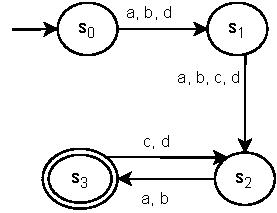
\includegraphics[height=100pt]{mintermization_automaton_m1.pdf}
        \caption{Finite automaton $A_1$ with transitions $\delta_1$.}
        \label{fig:diagram:mintermization_automaton_m1}
    \end{minipage}
    \hfill
    \begin{minipage}{0.49\linewidth}
        \centering
        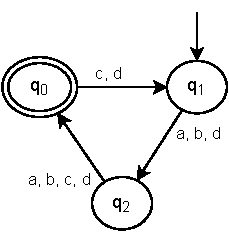
\includegraphics[height=100pt]{mintermization_automaton_m2.pdf}
        \caption{Finite automaton $A_2$ with transitions $\delta_2$.}
        \label{fig:diagram:mintermization_automaton_m2}
    \end{minipage}
    \vspace{0.5cm}
    \caption{Finite automata $A_1$ and $A_2$ used as example automata for mintermization.}
    \label{fig:diagram:mintermization_automata}
\end{figure*}

The Figure~\ref{fig:diagram:mintermization_automata_transition_sets} depicts how we could mark each transition set in our automata to be used in mintermization process. For example, a transition set $\varphi_1$ could be a set of transition symbols from state $s_0$ to $s_1$: $\varphi_i = {a, b, d}$. Similarly, we mark the remaining transition sets. Now, we can proceed to execute mintermization operations.

\begin{figure*}[ht]
    \centering
    \begin{minipage}{0.49\linewidth}
        \centering
        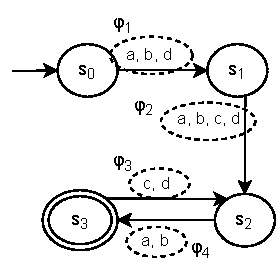
\includegraphics[height=100pt]{mintermization_automaton_m1_with_transition_sets.pdf}
        \caption{Finite automaton $A_1$ with transition sets $\varphi_i$.}
        \label{fig:diagram:mintermization_automaton_m1_with_transition_sets}
    \end{minipage}
    \hfill
    \begin{minipage}{0.49\linewidth}
        \centering
        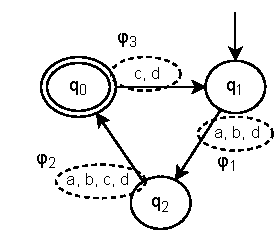
\includegraphics[height=100pt]{mintermization_automaton_m2_with_transition_sets.pdf}
        \caption{Finite automaton $A_2$ with transition sets $\varphi_i$.}
        \label{fig:diagram:mintermization_automaton_m2_with_transition_sets}
    \end{minipage}
    \vspace{0.5cm}
    \caption{Finite automata $A_1$ and $A_2$ with marked transition sets used in mintermization.}
    \label{fig:diagram:mintermization_automata_transition_sets}
\end{figure*}

If we were to compute minterms for these automata, we would proceed as follows: Starting with the whole alphabet of both automata\footnote{If the automata had non-equal alphabets, we would start with their intersection: $\Sigma = \Sigma_1 \cap \Sigma_2$} at the top of the minterm tree to be generated. Afterwards, we iterate over transition sets. For each transition set $\varphi_i$, we compute the intersection of the current minterm tree leaves with:
\begin{itemize}
    \item the current transition set $\varphi_i$ and store the result as a left node of this particular tree node,
    \item the complement of the current transition set $Q \setminus \varphi_i$ and store the result as a right tree node of this particular tree node.
\end{itemize}

If the intersection is empty, we omit creating the corresponding child node entirely. In the end, we are left with a complete minterm tree for the given set of transition sets $\Phi$ representing the specified finite automata.

The Figure~\ref{fig:diagram:mintermization_example} illustrates our mintermization process in a~diagram.

\begin{figure}[ht]
	\centering
	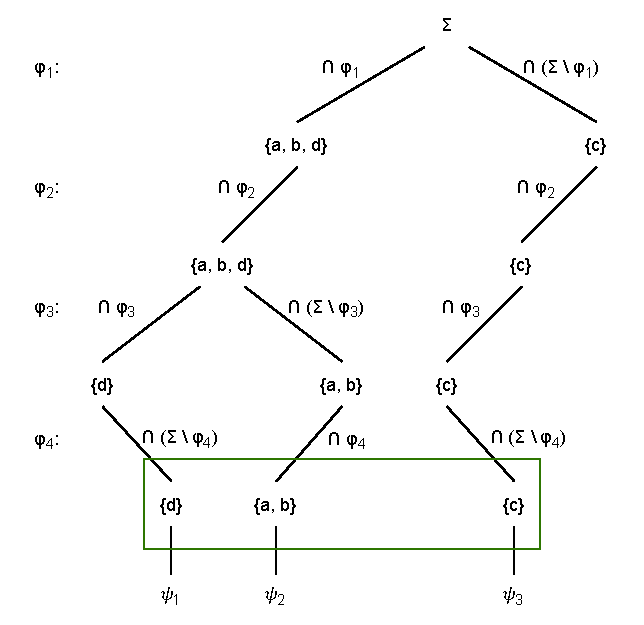
\includegraphics[]{mintermization_example.pdf}
	\caption{Mintermization process executed on example finite automata $A_1$ and $A_2$. We start with the whole alphabet and make our way down through all mintermization sets $\varphi_i$, where $1 \leq i \leq n$. For each mintermization set, we compute the intersection of the preceding set with the current mintermization set $\varphi_i$. The results are shown in the diagram as the nodes of the tree. When operations on all mintermization sets were executed, the leaves of the tree (indicated by the green square) represent the final minterms for the given mintermization sets $\Phi$ over the given alphabet $\Sigma$. We denote each minterm $\psi_i$, where $1 \leq i \leq |\Psi|$ where $|\Psi|$ represents the total number of generated minterms.}
	\label{fig:diagram:mintermization_example}
\end{figure}

The acquired minterms are:
$$ \Psi = Minterms(\Phi) = \{ \{d\}, \{a, b\}, \{c\} \} = \{ \psi_1, \psi_2, \psi_3 \} \text{.}$$

We can now substitute the former transition sets $\varphi_i$ for finite automata with the appropriate minterms $\psi_j, 1 \leq j \leq |\Psi|$ which were created from the specific transition sets $\varphi_i \in \Phi$ such that $\varphi_i$ is used in its direct form (not as a complement) in the process of computing $\psi_j$. The resulting automata can be seen in Figure~\ref{fig:diagram:mintermization_automata_with_minterms}.

\begin{figure*}[ht]
    \centering
    \begin{minipage}{0.49\linewidth}
        \centering
        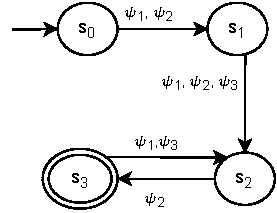
\includegraphics[height=100pt]{mintermization_automaton_m1_with_minterms.pdf}
        \caption{Finite automaton $A_1$ with transitions substituted by corresponding minterms $\psi_i \in \Psi$ created from these transition sets.}
        \label{fig:diagram:mintermization_automaton_m1_with_minterms}
    \end{minipage}
    \hfill
    \begin{minipage}{0.49\linewidth}
        \centering
        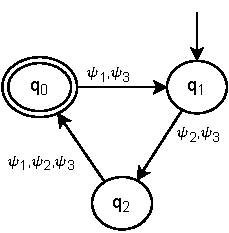
\includegraphics[height=100pt]{mintermization_automaton_m2_with_minterms.pdf}
        \caption{Finite automaton $A_2$ with transitions substituted by corresponding minterms $\psi_i \in \Psi$ created from these transition sets.}
        \label{fig:diagram:mintermization_automaton_m2_with_minterms}
    \end{minipage}
    \vspace{0.5cm}
    \caption{Finite automata $A_1$ and $A_2$ with substituted transitions with minterms in the process of mintermization.}
    \label{fig:diagram:mintermization_automata_with_minterms}
\end{figure*}

Consequently, assuming the previously said, considering we have minterms over alphabet of $A$, we know that the intersection of two minterms has to be an empty set and that $\forall \psi \in \Psi ( \psi \subseteq \varphi, \varphi \in \Phi )$ if $\psi$ is created from $\varphi$. We make use of this knowledge further.

In the following section, we propose a method of using minterm computation with Parikh image computation optimization. We choose this approach in order to mitigate the disadvantages of Parikh image computation for finite automata, especially those with multitude of transitions between two states varying only in transition symbols, which require considerate time to compute and evaluate. This method proceeds to represent such sets of transitions between two states with a single minterm representing these transitions. We can therefore apply any previously mentioned optimization methods (or any other known optimization method) on such modified automata with minterms as their transition symbols to construct their product without the need to compute, for example, Parikh image for every single transition symbol between two states. We can now compute possibly fewer transitions with the resulting minterms instead.

% TODO: Algorithm using minterms for computation methods.

%TODO

%--------------------------------------------------------
%--------------------------------------------------------
%--------------------------------------------------------
%--------------------------------------------------------
\chapter{Experiments and Results}\label{experimentsAndResultsChapter}

The reference implementation\footnote{In the \href{https://codeberg.org/Adda/optifa}{reference implementation}, we use \href{https://github.com/Z3Prover/z3}{Z3} as an SMT solver and automata operations are handled by \href{https://codeberg.org/Adda/symboliclib}{for our purposes modified library Symboliclib}.} of the proposed optimizations, written in Python 3, as well as a complete table of all of our experiments and their results and graphs is publicly accessible on a \href{https://codeberg.org/Adda/optifa}{Codeberg repository}\footnote{{\href{https://codeberg.org/Adda/optifa}{https://codeberg.org/Adda/optifa}}}. There is further explanation of the following graphs as well as additional graphs with description and in-depth analysis of performed experiments.

Test benchmarks used in our experiments were obtained from regular model checking. We have tested various different finite automata and their combinations. We have often used the same automata with their slightly changed variations to simulate real world examples of usually used automata to see how the optimized algorithm reduces the generated state space for certain types of automata with their typical qualities.

We have tested two main aspects:
\begin{itemize}
    \item First, we have tested the generated state space for emptiness test. That is, whenever we find a solution---final state in the intersection, the test ends, and we count the number of generated product states to this moment. If no intersection is found, we end the test when it is certain there is no final state and the intersection is indeed empty.
    \item Second, for the same pair of automata, we have tested the full product construction. Adding new final states along the way and comparing generated state spaces in the end for the full product accepting the whole intersection of original automata.
\end{itemize}

\section{Length Abstraction}

The following graphs show the results for both the emptiness test and full product construction. The graph in Figure~\ref{fig:graph:et_state_space_sizes_comp} shows the comparison of product state spaces sizes in basic product construction algorithm and our optimized algorithm considering length abstraction for emptiness test. Sorted in order of increasing product state space size generated by the basic product construction algorithm. The graph in Figure~\ref{fig:graph:fp_state_space_sizes_comp} shows the same data, only for the full product construction experiment.

\begin{figure*}[ht]
    \centering
    \begin{minipage}{0.49\linewidth}
        \centering
        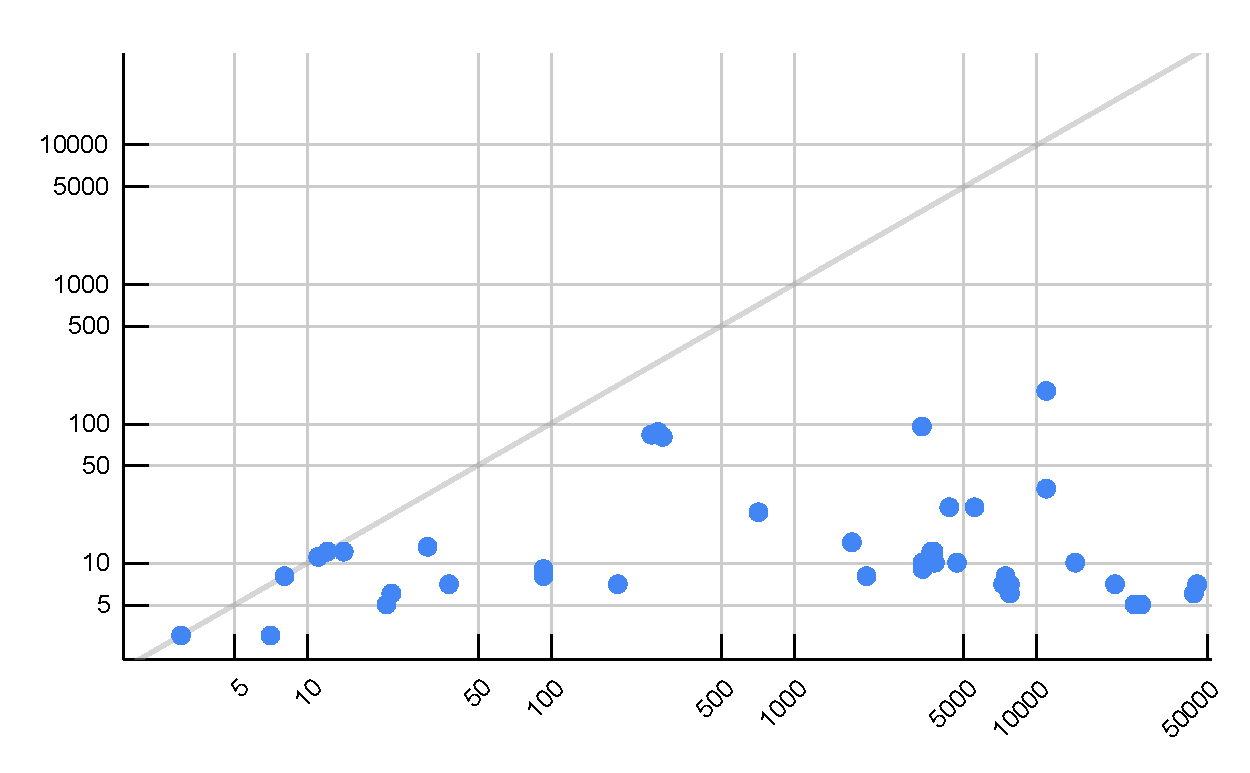
\includegraphics[width=\linewidth]{graph_scatter_et.pdf}
        \caption{Emptiness test}
        \label{fig:graph:et_state_space_sizes_comp}
    \end{minipage}
    \hfill
    \begin{minipage}{0.49\linewidth}
        \centering
        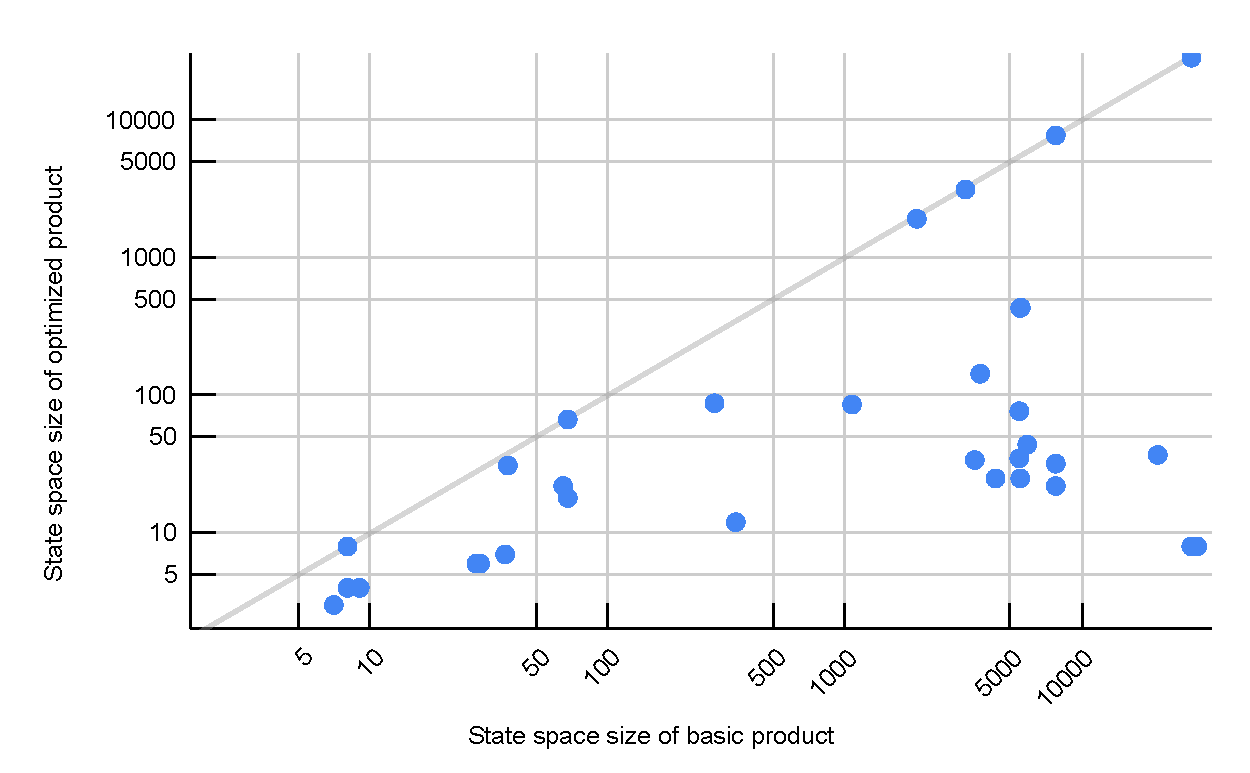
\includegraphics[width=\linewidth]{graph_scatter_fp.pdf}
        \caption{Full product construction}
        \label{fig:graph:fp_state_space_sizes_comp}
    \end{minipage}
    \vspace{0.5cm}
    \caption{Comparison of state space sizes generated by basic and optimized product construction algorithms. Both axes are in logarithmic scale, x-axis showing state space sizes of basic product, y-axis state space sizes of optimized product.}
    \label{fig:graph:product_state_space_sizes}
\end{figure*}

Where the length abstraction cannot optimize the product construction, both products have about the same state space size. These results are caused mostly by constructing products of two almost identical automata with only a few states/transitions missing/added which do not affect the accepting runs for recognized languages. There are therefore no branches which can be trimmed---most of the processed states are evaluated as \emph{satisfiable} in length abstraction satisfiability check. In full product construction results, if there are nearly no product states to trim, the generated product state space size \emph{explodes} similarly to the basic product construction algorithm---typical for automata with large numbers of transitions from every state causing large numbers of possible accepted lengths, where our algorithm can trim only a few states.

For another automata, the product generated by our algorithm is much smaller. We can see from the graphs that the larger the basic product state space size gets, the higher impact our optimization has on the product state space size. The same holds for the full product construction results. For cases where the intersection is truly empty and accepted lengths differ in both automata, our algorithm stops the process of product construction on the very first tested product state. The basic algorithm continues to create a full product.

We get the best results for automata with practically the same transitions which differ only slightly in final states or a few transitions which affects the accepting runs in the original automata. These changes cause the basic algorithm to generate the product states without realizing most (if not all) product states do not lead to a final state. These slight differences in automata (especially in final states) usually also change the length of accepted words. Therefore, our optimization is able to notice these differences and trim most of the product state space, if not the whole product, when no final state can be accessed and the intersection is empty.

In both graphs, we can see the aforementioned quadratic state space explosion for product is nearly not affecting our algorithm in comparison to the basic product construction algorithm. Optimized products are easier to work with and operations on such products require less computational time and memory consumption.

It is worth mentioning that we have neglected the number of generated state space for our lasso automata this whole time. We can use deterministic minimization on original automata to further optimize the generated state space for lasso automata and products. However, we do not need these lasso automata after product construction is complete. Therefore, the lasso automata do not affect how efficiently we work with the generated product. Nevertheless, the number of generated lasso states in the process of deciding the intersection emptiness test matters. For different automata, the generated state space varies. For state space sizes of lasso automata in our experiments, see \href{https://codeberg.org/Adda/optifa/src/branch/master/results}{Codeberg repository}\footnote{{\href{https://codeberg.org/Adda/optifa/src/branch/master/results}{https://codeberg.org/Adda/optifa/src/branch/master/results}}}.

\begin{figure*}[ht]
    \centering
    \begin{minipage}{0.49\linewidth}
        \centering
        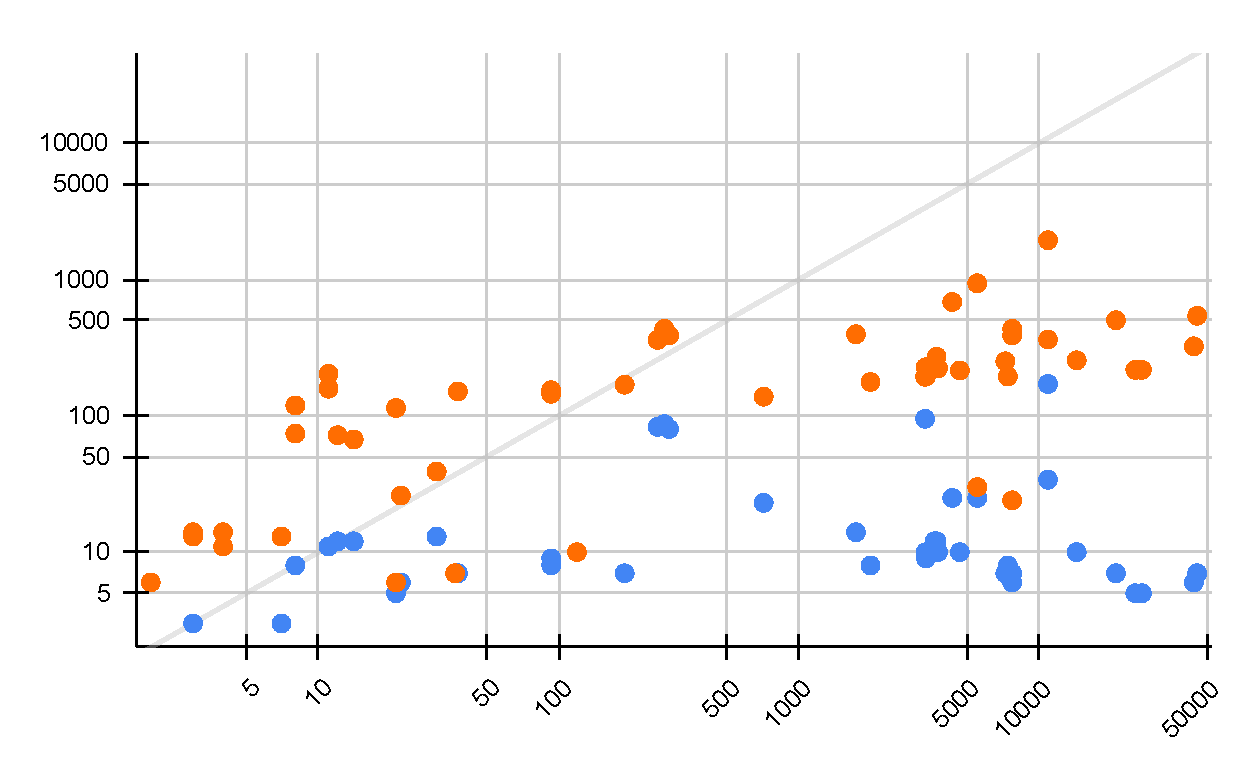
\includegraphics[width=\linewidth]{graph_scatter_combined_et.pdf}
        \caption{Emptiness test}
        \label{fig:graph:et_state_space_sizes_comp_with_lasso}
    \end{minipage}
    \hfill
    \begin{minipage}{0.49\linewidth}
        \centering
        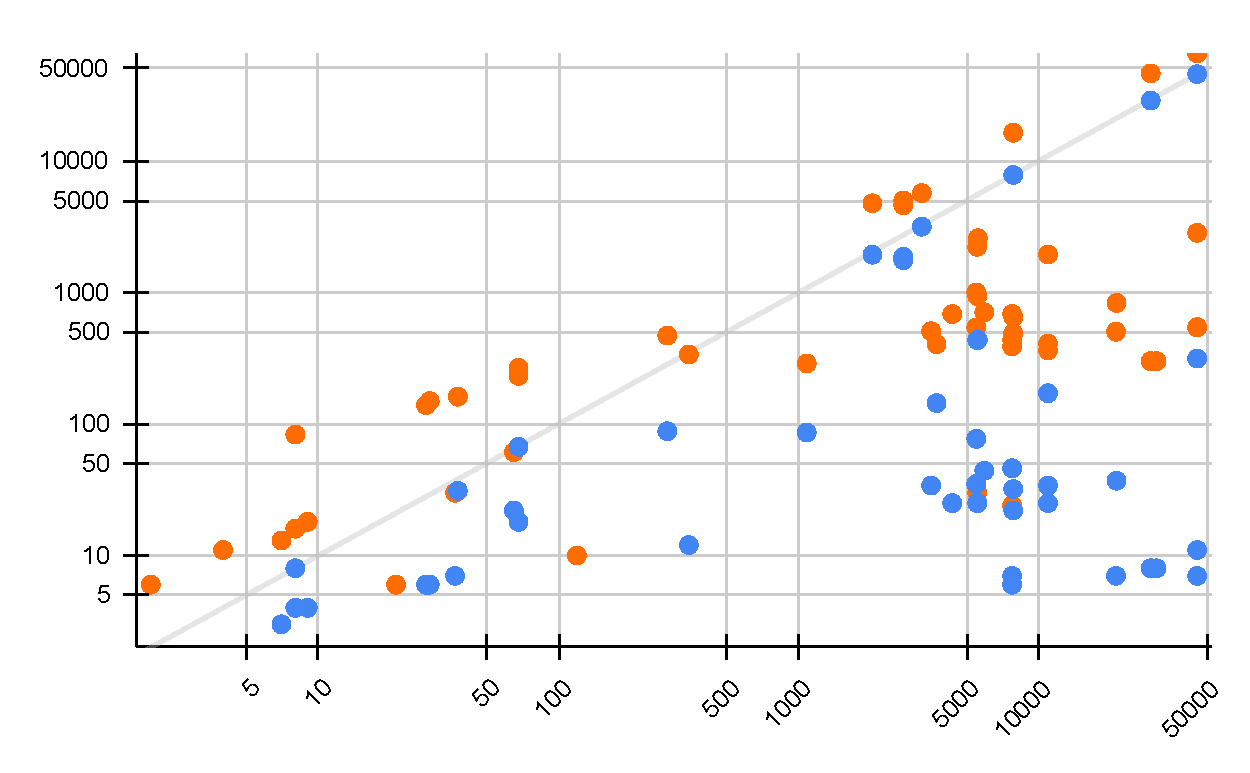
\includegraphics[width=\linewidth]{graph_scatter_combined_fp.pdf}
        \caption{Full product construction}
        \label{fig:graph:fp_state_space_sizes_comp_with_lasso}
    \end{minipage}
    \vspace{0.5cm}
    \caption{Comparison of state space sizes generated by basic and optimized product construction algorithms with sum of states generated for both the final optimized product and lasso automata states generated in the process of the product construction. Both axes are in logarithmic scale, x-axis showing state space sizes of basic product, y-axis state space sizes of optimized product (and optimized product with lasso automata states). The blue dots represent only the optimized product state space sizes (as in Figure~\ref{fig:graph:product_state_space_sizes}), the orange dots the sum of optimized product state space sizes and the generated lasso states.}
    \label{fig:graph:product_state_space_sizes_with_lasso}
\end{figure*}

As we can see in Figure~\ref{fig:graph:product_state_space_sizes_with_lasso}, even when counting with lasso automata product state space sizes, the total number of generated states in the whole process of the product construction is usually lower than the basic product state space size. The larger the automata are, the better results we get. It is understandable, that for smaller original automata, whose intersection is computed, the expense of generating lasso automata is significant in comparison with the generated product state space sizes. The larger the original automata get, the lesser the expense of the number of lasso automata states is in comparison with the basic product state space.

\begin{figure*}[ht]
    \centering
    \begin{minipage}{0.49\linewidth}
        \centering
        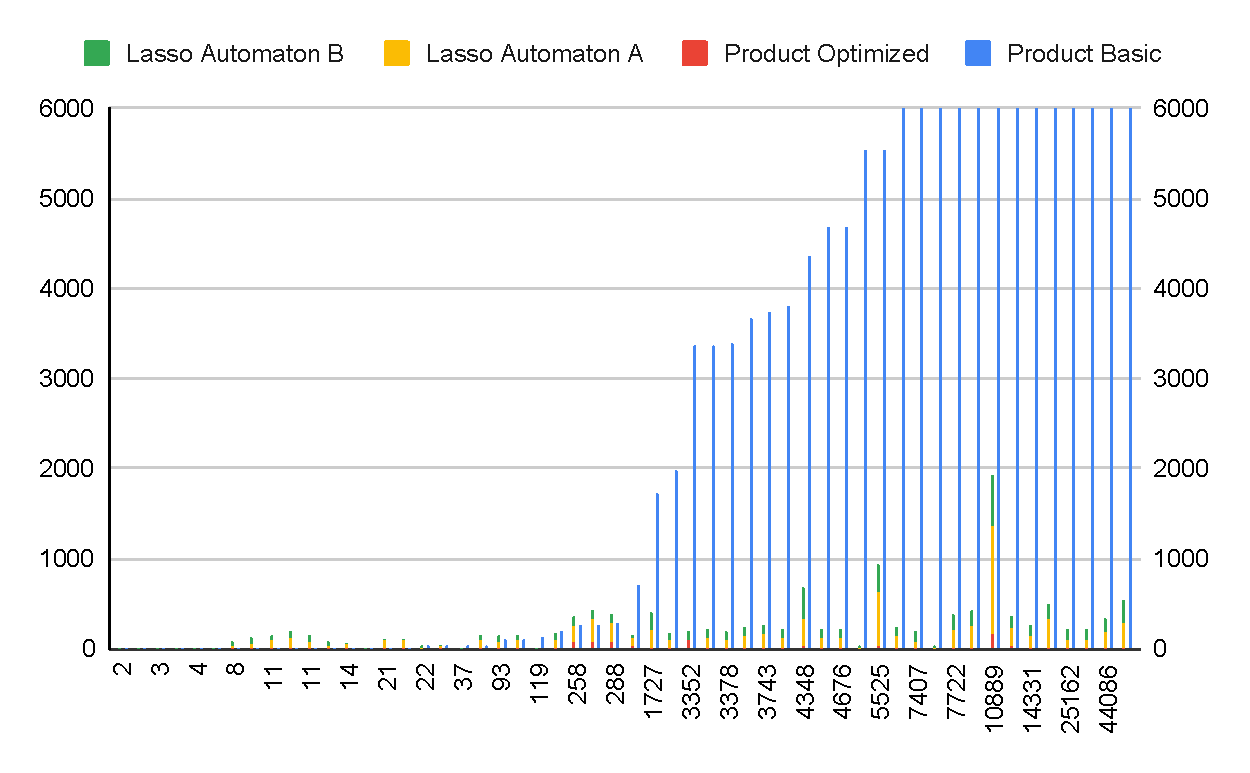
\includegraphics[width=\linewidth]{graph_stacked_et.pdf}
        \caption{Emptiness test}
        \label{fig:graph:stacked_et_state_space_sizes_comp_with_lasso}
    \end{minipage}
    \hfill
    \begin{minipage}{0.49\linewidth}
        \centering
        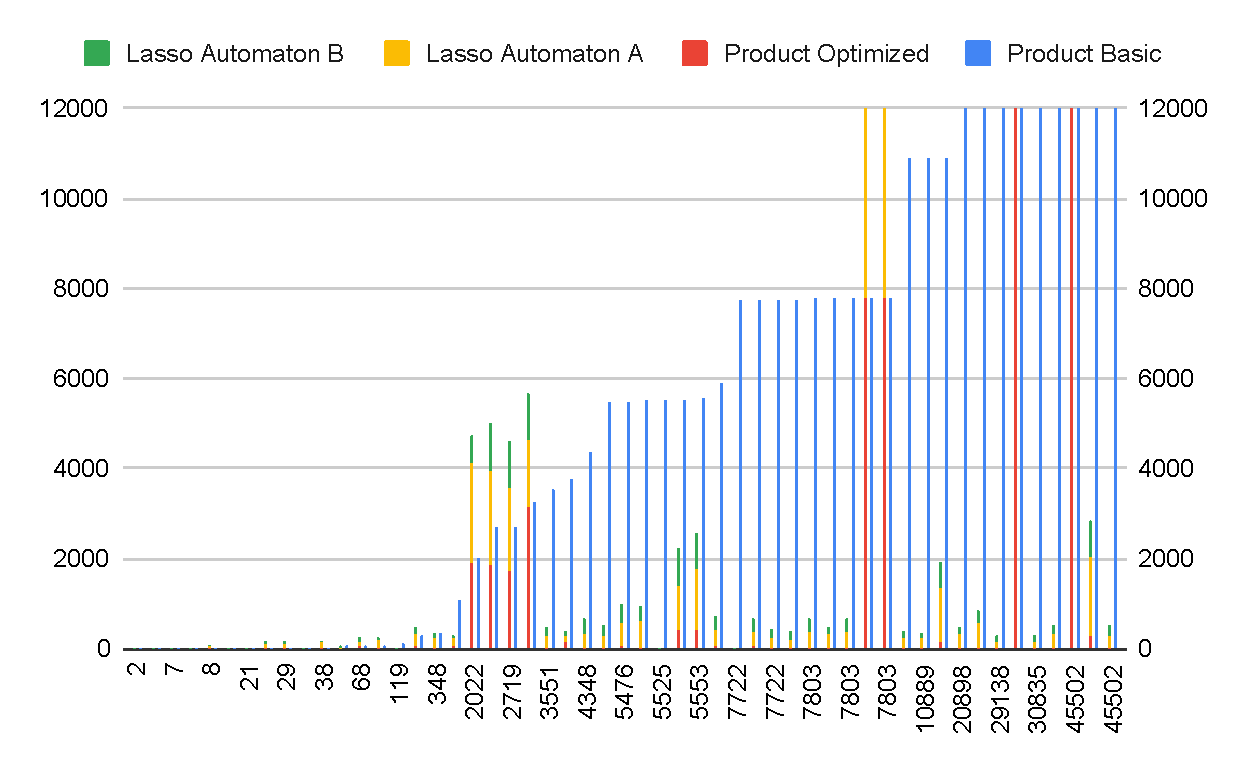
\includegraphics[width=\linewidth]{graph_stacked_fp.pdf}
        \caption{Full product construction}
        \label{fig:graph:stacked_fp_state_space_sizes_comp_with_lasso}
    \end{minipage}
    \vspace{0.5cm}
    \caption{Stacked comparison of state space sizes generated by basic and optimized product construction algorithms with sum of states generated for both the final optimized product and lasso automata states generated in the process of the product construction. Both axes are in logarithmic scale, x-axis showing state space sizes of basic product (ordered in ascending order), y-axis state space sizes of depicted experiments---because of huge differences in sizes of basic product and optimized product with lasso automata, the largest shown values are set to 6000 and 12000, respectively. Each two columns show a single experiment with our optimized solution as the left (green, red, and orange) column---as a sum of all generated states (of optimized product (green) and both lasso automata (red and orange), and the right blue column as the basic product state space size).}
    \label{fig:graph:stacked_product_state_space_sizes_with_lasso}
\end{figure*}

Out of all experiments, one weakness of our algorithm is clear---the more final states the original automata have, the more difficult it is to optimize the full product construction using length abstraction. This is caused by the fact that every final state increases the number of accepted different lengths per automaton. Therefore, with automata where out of hundreds or thousands of states nearly every state is a final state too, our optimization algorithm has to consider multiple possible lengths and cannot easily determine which branches will not be accepted by the product automaton.

\section{Parikh Image Computation}

In this section, we show results of several experiments with Parikh image computation optimization. At first, we are interested in pruning capabilities of Parikh image abstraction without further optimizations. Later, we provide results for introduced optimizations of Parikh image computation algorithm.

The following graphs show the results for both the emptiness test and full product construction of unoptimized Parikh image computation abstraction. The graph in Figure~\ref{fig:graph:pi_et_state_space_sizes_comp} shows the comparison of product state spaces sizes in basic product construction algorithm and our Parikh image computation algorithm for emptiness test. Sorted in order of increasing product state space size generated by the basic product construction algorithm. The graph in Figure~\ref{fig:graph:pi_fp_state_space_sizes_comp} shows the same data, only for the full product construction experiment.

\begin{figure*}[ht]
    \centering
    \begin{minipage}{0.49\linewidth}
        \centering
        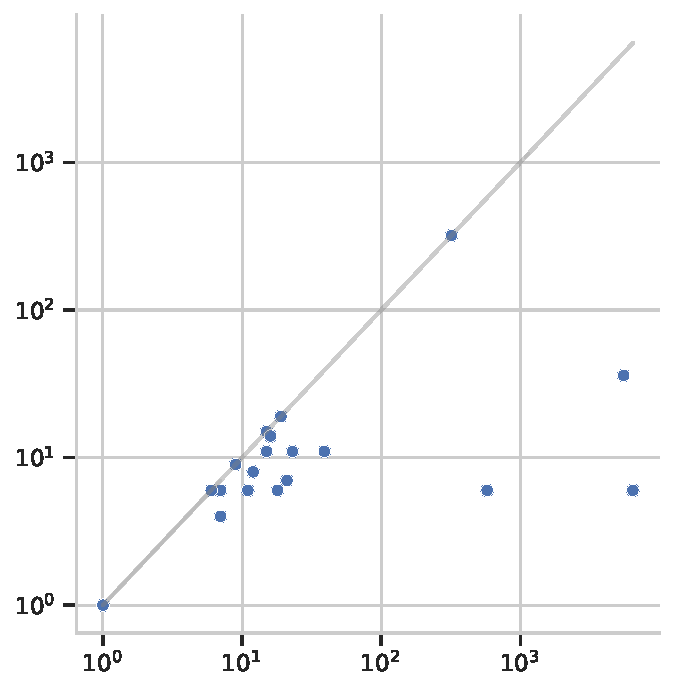
\includegraphics[height=150pt]{graph_pi_et_scatter.pdf}
        \caption{Emptiness test}
        \label{fig:graph:pi_et_state_space_sizes_comp}
    \end{minipage}
    \hfill
    \begin{minipage}{0.49\linewidth}
        \centering
        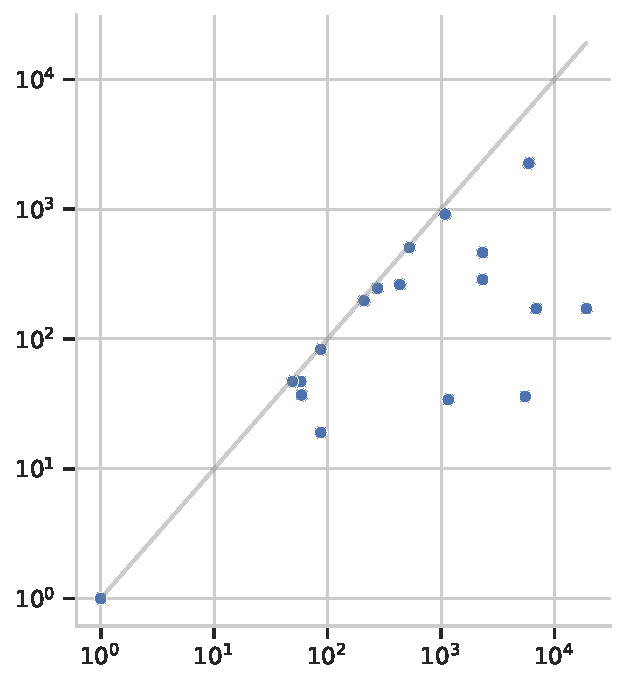
\includegraphics[height=150pt]{graph_pi_fp_scatter.pdf}
        \caption{Full product construction}
        \label{fig:graph:pi_fp_state_space_sizes_comp}
    \end{minipage}
    \vspace{0.5cm}
    \caption{Comparison of state space sizes generated by basic and optimized with Parikh image computation product construction algorithms. Both axes are in logarithmic scale, x-axis showing state space sizes of basic product, y-axis state space sizes of optimized product.}
    \label{fig:graph:pi_product_state_space_sizes}
\end{figure*}

We conclude from the experiments that Parikh image optimizes the generated product state space in nearly every case. The strength of Parikh image is its higher pruning capacity due to wider range of information gathered from the automata. In multiple cases, Parikh image optimization is able to prune vast \emph{branches} of potential generated product by correctly determining incompatible transition symbols even if possible lengths of accepted words are mutually compatible.

Incremental SMT solving proves to be a great improvement to the Parikh image computation optimization. The amount of clauses depends on the number of states in finite automata, the number of transitions and the number of initial or final states. See Table~\ref{table:incremental_smt_clauses} for a depiction of comparison of the number of all clauses in Parikh image, clauses common to all product states (persistent clauses) and state specific clauses.

\begin{table*}[ht]
	\centering
    \begin{tabular}{ |c|c|c|c|c| }
        \hline
        Product States & All Clauses & Persistent Clauses & State Specific Clauses & Ratio \\ \hline
        434 & 2652 & 1782 & 870 & 67.2\% \\ \hline
    \end{tabular}
    \caption{An example proportion of persistent and state specific clauses in Parikh image computation with incremental SMT solving optimization. The \emph{Product States} column shows the number of product states in the whole intersection product, the \emph{All Clauses} column shows the number of clauses in each computed Parikh image, the \emph{Persistent Clauses} column shows the number of persistent clauses in the whole Parikh image (out of the all Parikh image clauses), \emph{State Specific Clauses} column states how many Parikh image clauses have to be recomputed for each product state and \emph{Ratio} column shows the ratio of persistent clauses in all Parikh image clauses.}
    \label{table:incremental_smt_clauses}
\end{table*}

We can notice that the number of persistent clauses covers substantial part of all Parikh image clauses (experimentally determined to be usually around $70 \%$ for our benchmark automata). Therefore, around $70\%$ of each computed Parikh image clauses can be precomputed once. Only $30\%$ of clauses must be computed repeatedly for each potential product state.

\section{Combination of State Language Abstractions}

We show results of several experiments with Parikh image computation optimization. At first, we are interested in pruning capabilities of Parikh image abstraction without further optimizations. Later, we provide results for introduced optimizations of Parikh image computation algorithm.

The following graphs in Figure~\ref{fig:graph:pi_product_state_space_sizes} show the results for both the emptiness test and full product construction of unoptimized Parikh image computation abstraction. The graph in Figure~\ref{fig:graph:pi_et_state_space_sizes_comp} shows the comparison of product state spaces sizes in basic product construction algorithm and our Parikh image computation algorithm for emptiness test. Sorted in order of increasing product state space size generated by the basic product construction algorithm. The graph in Figure~\ref{fig:graph:pi_fp_state_space_sizes_comp} shows the same data, only for the full product construction experiment.

%\begin{figure}[ht]
%    \centering
%        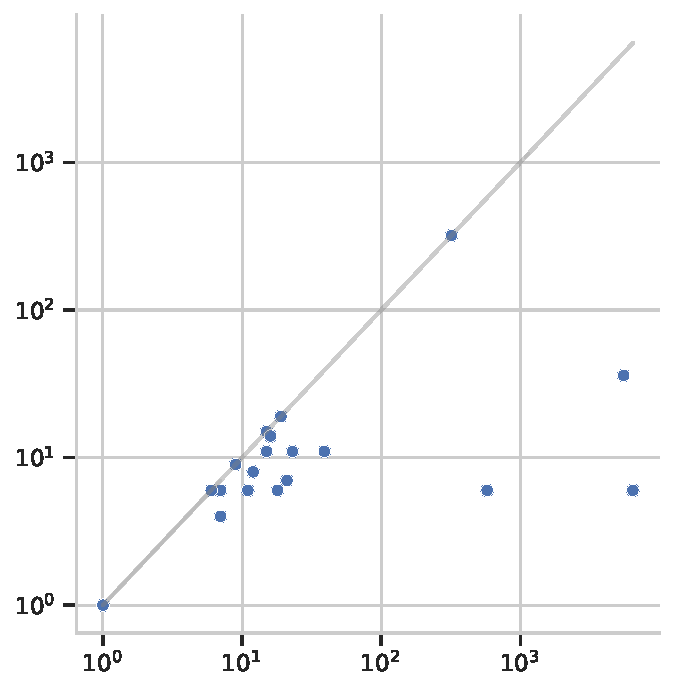
\includegraphics[height=100pt]{graph_pi_et_scatter.pdf}
%        \caption{Emptiness test}
%        \label{fig:graph:pi_et_state_space_sizes_comp}
%        \vspace{0.4cm}
%        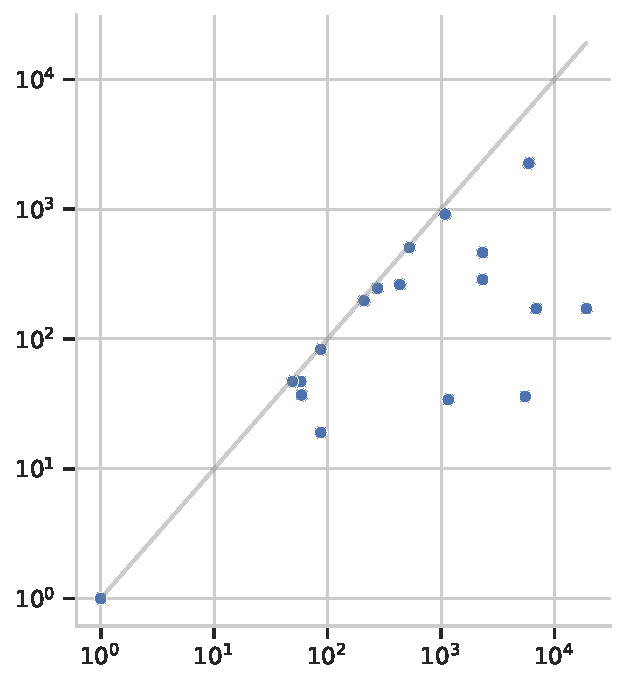
\includegraphics[height=100pt]{graph_pi_fp_scatter.pdf}
%        \caption{Full product construction}
%        \label{fig:graph:pi_fp_state_space_sizes_comp}
%    \vspace{0.4cm}
%    \caption{Comparison of state space sizes generated by basic and optimized with Parikh image computation product construction algorithms. Both axes are in logarithmic scale, x-axis showing state space sizes of basic product, y-axis state space sizes of optimized product.}
%    \label{fig:graph:pi_product_state_space_sizes}
%\end{figure}

\begin{figure}[ht]
    \centering
    \begin{minipage}{0.49\linewidth}
        \centering
        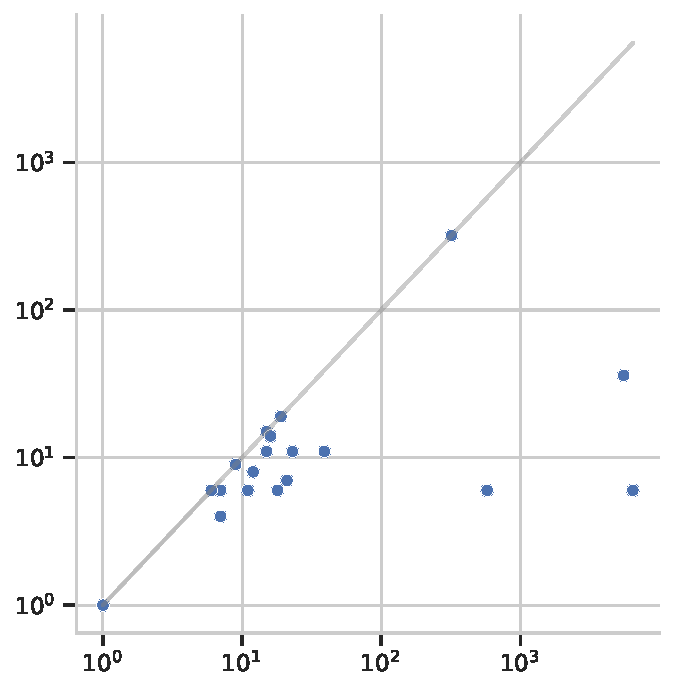
\includegraphics[height=120pt]{graph_pi_et_scatter.pdf}
        \caption{Emptiness test}
        \label{fig:graph:pi_et_state_space_sizes_comp}
    \end{minipage}
    \hfill
    \begin{minipage}{0.49\linewidth}
        \centering
        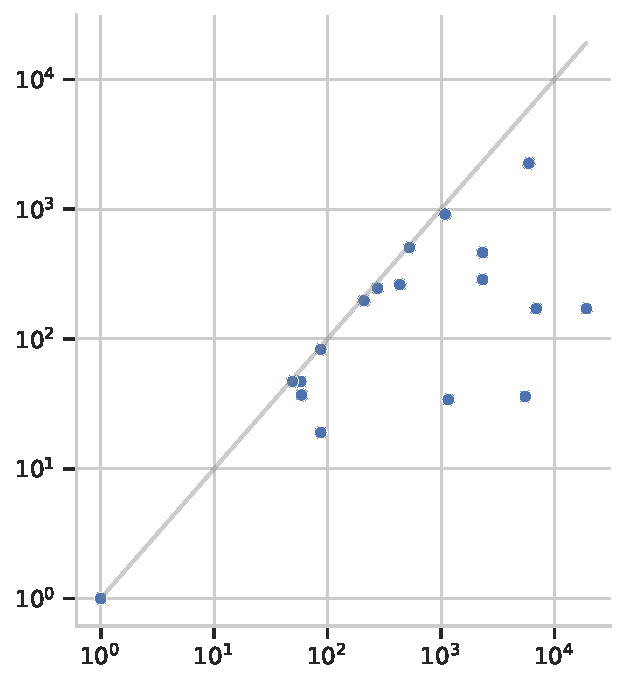
\includegraphics[height=120pt]{graph_pi_fp_scatter.pdf}
        \caption{Full product}
        \label{fig:graph:pi_fp_state_space_sizes_comp}
    \end{minipage}
    \vspace{0.5cm}

    \caption{Comparison of state space sizes generated by basic and optimized product construction algorithms with length abstraction (blue dots) and Parikh image computation (orange dots). Both axes are in symmetrical logarithmic scale\protect\footnotemark, showing state space sizes: x-axis of basic product, y-axis of optimized product.}
    \label{fig:graph:pi_product_state_space_sizes}
\end{figure}

\footnotetext{Plot is linear around $0$ instead of logarithmic.}

We conclude from the experiments that Parikh image optimizes the generated product state space in nearly every case and produces equal or better results than length abstraction every time. The strength of Parikh image is its higher pruning capacity due to wider range of information gathered from the automata. In multiple cases, Parikh image optimization is able to prune vast \emph{branches} of potential generated product by correctly determining incompatible transition symbols even if possible lengths of accepted words are mutually compatible, sometimes even entirely stopping product construction immediately when basic and length abstraction constructions continue to generate state space further.

Incremental SMT solving proves to be a great improvement to the Parikh image computation optimization. The amount of clauses depends on the number of states in finite automata, the number of transitions and the number of initial or final states. The following experiment provides an example comparison of the number of all clauses in Parikh image, clauses common to all product states (persistent clauses) and state specific clauses. For a product of $434$ states, each product state Parikh image contains $2652$ clauses. From those, $1782$ clauses are persistent clauses and the remaining $870$ are state specific clauses. A proportional ratio o persistent clauses in whole Parikh image is around $67.2 \%$. The number of persistent clauses (experimentally determined to be usually around $70 \%$) for our benchmark automata means around $70\%$ of each computed Parikh image clauses can be precomputed once. Only $30\%$ of clauses must be computed repeatedly for each potential product state.

%--------------------------------------------------------
%--------------------------------------------------------
%--------------------------------------------------------
%--------------------------------------------------------
\chapter{Conclusion}

The most demanding parts of the intersection computation is the generation of product states and transitions of the product automaton. We tried to reduce the size of the generated state space by omitting the states which cannot lead to any final state---that is, omitting the \textit{branches} which do not lead to any final state---by performing the emptiness test of such states using various state languages abstractions over the original automata such as length abstraction using lasso automata or Parikh image computation based on Parikh's theorem. Each approach has been experimentally tested and further optimizations to the proposed algorithms were introduced.

According to our experiments, product state space is minimized especially for intersections with huge non-terminating branches or for intersections of automata accepting different lengths of words recognized by the automata languages. Further, for automata with long lines and similar automata varying only slightly from each other. Experiments show our algorithm generates smaller product state spaces for both emptiness test and full product construction, which are two usually used operations on automata intersection. All our abstractions consider over-approximation of possible products. Therefore, our optimizations are safe to use for any uses resolving operations on finite automata.

We have not encountered similar approaches to product construction optimization using length abstraction or Parikh image computation to compare our results with. It might be worth investing into combining our orthogonal approach with other existing algorithms to see how the generated product state space is affected. We are talking about abstraction techniques such as CEGAR~\cite{DBLP:conf/cav/ClarkeGJLV00} and predicate abstraction~\cite{DBLP:conf/cav/ColonU98, DBLP:conf/cav/GrafS97}, IMPACT~\cite{DBLP:conf/cav/McMillan06}, possibly IC3/PDR~\cite{DBLP:conf/sat/HoderB12, DBLP:conf/fmcad/BradleyM07}. All the above techniques have proven efficient in hardware or software verification, and they can be applied in automata too. First attempts to use these techniques in finite automata problem-solving are based on IC3~\cite{DBLP:journals/pacmpl/HolikJLRV18, DBLP:conf/cav/WangTLYJ16, DBLP:journals/corr/abs-1708-09073} and on the interpolation-based approach of McMillan~\cite{DBLP:conf/tacas/AmlaM07, DBLP:conf/tacas/GangeNSSS13}.
